\documentclass[twoside]{book}

% Packages required by doxygen
\usepackage{fixltx2e}
\usepackage{calc}
\usepackage{doxygen}
\usepackage[export]{adjustbox} % also loads graphicx
\usepackage{graphicx}
\usepackage[utf8]{inputenc}
\usepackage{makeidx}
\usepackage{multicol}
\usepackage{multirow}
\PassOptionsToPackage{warn}{textcomp}
\usepackage{textcomp}
\usepackage[nointegrals]{wasysym}
\usepackage[table]{xcolor}

% Font selection
\usepackage[T1]{fontenc}
\usepackage[scaled=.90]{helvet}
\usepackage{courier}
\usepackage{amssymb}
\usepackage{sectsty}
\renewcommand{\familydefault}{\sfdefault}
\allsectionsfont{%
  \fontseries{bc}\selectfont%
  \color{darkgray}%
}
\renewcommand{\DoxyLabelFont}{%
  \fontseries{bc}\selectfont%
  \color{darkgray}%
}
\newcommand{\+}{\discretionary{\mbox{\scriptsize$\hookleftarrow$}}{}{}}

% Page & text layout
\usepackage{geometry}
\geometry{%
  a4paper,%
  top=2.5cm,%
  bottom=2.5cm,%
  left=2.5cm,%
  right=2.5cm%
}
\tolerance=750
\hfuzz=15pt
\hbadness=750
\setlength{\emergencystretch}{15pt}
\setlength{\parindent}{0cm}
\setlength{\parskip}{3ex plus 2ex minus 2ex}
\makeatletter
\renewcommand{\paragraph}{%
  \@startsection{paragraph}{4}{0ex}{-1.0ex}{1.0ex}{%
    \normalfont\normalsize\bfseries\SS@parafont%
  }%
}
\renewcommand{\subparagraph}{%
  \@startsection{subparagraph}{5}{0ex}{-1.0ex}{1.0ex}{%
    \normalfont\normalsize\bfseries\SS@subparafont%
  }%
}
\makeatother

% Headers & footers
\usepackage{fancyhdr}
\pagestyle{fancyplain}
\fancyhead[LE]{\fancyplain{}{\bfseries\thepage}}
\fancyhead[CE]{\fancyplain{}{}}
\fancyhead[RE]{\fancyplain{}{\bfseries\leftmark}}
\fancyhead[LO]{\fancyplain{}{\bfseries\rightmark}}
\fancyhead[CO]{\fancyplain{}{}}
\fancyhead[RO]{\fancyplain{}{\bfseries\thepage}}
\fancyfoot[LE]{\fancyplain{}{}}
\fancyfoot[CE]{\fancyplain{}{}}
\fancyfoot[RE]{\fancyplain{}{\bfseries\scriptsize Generated by Doxygen }}
\fancyfoot[LO]{\fancyplain{}{\bfseries\scriptsize Generated by Doxygen }}
\fancyfoot[CO]{\fancyplain{}{}}
\fancyfoot[RO]{\fancyplain{}{}}
\renewcommand{\footrulewidth}{0.4pt}
\renewcommand{\chaptermark}[1]{%
  \markboth{#1}{}%
}
\renewcommand{\sectionmark}[1]{%
  \markright{\thesection\ #1}%
}

% Indices & bibliography
\usepackage{natbib}
\usepackage[titles]{tocloft}
\setcounter{tocdepth}{3}
\setcounter{secnumdepth}{5}
\makeindex

% Hyperlinks (required, but should be loaded last)
\usepackage{ifpdf}
\ifpdf
  \usepackage[pdftex,pagebackref=true]{hyperref}
\else
  \usepackage[ps2pdf,pagebackref=true]{hyperref}
\fi
\hypersetup{%
  colorlinks=true,%
  linkcolor=blue,%
  citecolor=blue,%
  unicode%
}

% Custom commands
\newcommand{\clearemptydoublepage}{%
  \newpage{\pagestyle{empty}\cleardoublepage}%
}

\usepackage{caption}
\captionsetup{labelsep=space,justification=centering,font={bf},singlelinecheck=off,skip=4pt,position=top}

%===== C O N T E N T S =====

\begin{document}

% Titlepage & ToC
\hypersetup{pageanchor=false,
             bookmarksnumbered=true,
             pdfencoding=unicode
            }
\pagenumbering{alph}
\begin{titlepage}
\vspace*{7cm}
\begin{center}%
{\Large Stoched\+: A\+PC 524 Final Project }\\
\vspace*{1cm}
{\large Generated by Doxygen 1.8.13}\\
\end{center}
\end{titlepage}
\clearemptydoublepage
\pagenumbering{roman}
\tableofcontents
\clearemptydoublepage
\pagenumbering{arabic}
\hypersetup{pageanchor=true}

%--- Begin generated contents ---
\chapter{Stoched}
\label{index}\hypertarget{index}{}\subsubsection*{Introduction}

Stoched$\ast$ is a platform for simulating realizations of stochastic systems modeled by rate equations. The Gillespie algorithm performs exact simulations. Also, more scalable approximate algorithms derived from the Gillespie algorithm are useful for large systems. These algorithms have historically been used to solve problems in molecular dynamics; today, they are applied to a wide variety of stochastic modeling problems. The platform is a fast, compiled code tool with an extremely simple interface aimed towards scientists with minimal programming experience. While other tools for stochastic modeling and simulation exist, none have non-\/programmer-\/friendly interfaces and few are specialized to those systems modeled by rate equations alone. We take user-\/friendly modeling languages developed for Bayesian inference (B\+U\+G\+S/\+J\+A\+GS and Stan) as guides.

\subsubsection*{License}

Permission to use, copy, modify, and distribute this software and its documentation under the terms of the G\+NU General Public License is hereby granted. No representations are made about the suitability of this software for any purpose. It is provided \char`\"{}as is\char`\"{} without express or implied warranty. See the G\+NU General Public License for more details.

Documents produced by Stoched are derivative works derived from the input used in their production; they are not affected by this license.

\subsubsection*{Links}

\href{https://www.gnu.org/software/bison/}{\tt Flex/\+Bison}

\href{https://www.open-mpi.org/}{\tt Open M\+PI} 
\chapter{R\+E\+A\+D\+ME}
\label{md___users__caleb__a_p_c524_stoched_src__r_e_a_d_m_e}
\Hypertarget{md___users__caleb__a_p_c524_stoched_src__r_e_a_d_m_e}
\#source code 
\chapter{Hierarchical Index}
\section{Class Hierarchy}
This inheritance list is sorted roughly, but not completely, alphabetically\+:\begin{DoxyCompactList}
\item \contentsline{section}{Event}{\pageref{class_event}}{}
\item \contentsline{section}{Model}{\pageref{class_model}}{}
\item \contentsline{section}{Paramset}{\pageref{class_paramset}}{}
\item \contentsline{section}{Realization}{\pageref{class_realization}}{}
\begin{DoxyCompactList}
\item \contentsline{section}{Euler\+Leap}{\pageref{class_euler_leap}}{}
\item \contentsline{section}{First\+Reaction}{\pageref{class_first_reaction}}{}
\item \contentsline{section}{Midpoint\+Leap}{\pageref{class_midpoint_leap}}{}
\item \contentsline{section}{Next\+Reaction}{\pageref{class_next_reaction}}{}
\end{DoxyCompactList}
\item \contentsline{section}{Realization\+Factory}{\pageref{class_realization_factory}}{}
\item \contentsline{section}{rng}{\pageref{classrng}}{}
\begin{DoxyCompactList}
\item \contentsline{section}{xoroshiro128plus}{\pageref{classxoroshiro128plus}}{}
\end{DoxyCompactList}
\end{DoxyCompactList}

\chapter{Class Index}
\section{Class List}
Here are the classes, structs, unions and interfaces with brief descriptions\+:\begin{DoxyCompactList}
\item\contentsline{section}{\hyperlink{class_euler_leap}{Euler\+Leap} \\*Class \hyperlink{class_euler_leap}{Euler\+Leap} implements \hyperlink{class_realization}{Realization} step() function using Euler Leap method }{\pageref{class_euler_leap}}{}
\item\contentsline{section}{\hyperlink{class_event}{Event} \\*Class \hyperlink{class_event}{Event} holds a user-\/specified event, namely set of functions and associated rate }{\pageref{class_event}}{}
\item\contentsline{section}{\hyperlink{class_first_reaction}{First\+Reaction} \\*Class \hyperlink{class_first_reaction}{First\+Reaction} takes first \hyperlink{class_first_reaction_aed63c3c95d20b2ad557dabb6c5376a73}{step()} according to chosen algorithm }{\pageref{class_first_reaction}}{}
\item\contentsline{section}{\hyperlink{class_model}{Model} \\*Class \hyperlink{class_model}{Model}, which holds user-\/specified models of stochastic systems from which realizations are to be simulated. A model may have variable parameters; each complete set will be stored in an object of class \hyperlink{class_paramset}{Paramset} }{\pageref{class_model}}{}
\item\contentsline{section}{\hyperlink{class_next_reaction}{Next\+Reaction} \\*Class \hyperlink{class_first_reaction}{First\+Reaction} takes next \hyperlink{class_next_reaction_a2c1502879c76efe398c2947056936725}{step()} according to chosen algorithm }{\pageref{class_next_reaction}}{}
\item\contentsline{section}{\hyperlink{class_paramset}{Paramset} \\*Class \hyperlink{class_paramset}{Paramset} holds a particular set of pameters for user requested simulation run(s) }{\pageref{class_paramset}}{}
\item\contentsline{section}{\hyperlink{class_realization}{Realization} \\*Class \hyperlink{class_realization}{Realization} holds realizations of a \hyperlink{class_model}{Model} (state array, propensities, waiting times, etc.) }{\pageref{class_realization}}{}
\item\contentsline{section}{\hyperlink{class_realization_factory}{Realization\+Factory} \\*Class \hyperlink{class_realization_factory}{Realization\+Factory} generates required instance of \hyperlink{class_realization}{Realization} (\hyperlink{class_first_reaction}{First\+Reaction}, \hyperlink{class_next_reaction}{Next\+Reaction}, \hyperlink{class_euler_leap}{Euler\+Leap}) based on input }{\pageref{class_realization_factory}}{}
\item\contentsline{section}{\hyperlink{classrng}{rng} \\*Class rng implements random number generator, based upon public domain xorshift implementations by David Blackman and Sebastiano Vigna (\href{mailto:vigna@acm.org}{\tt vigna@acm.\+org}) }{\pageref{classrng}}{}
\item\contentsline{section}{\hyperlink{classxoroshiro128plus}{xoroshiro128plus} \\*Class \hyperlink{classxoroshiro128plus}{xoroshiro128plus} implements a random number generator of Class rng }{\pageref{classxoroshiro128plus}}{}
\end{DoxyCompactList}

\chapter{File Index}
\section{File List}
Here is a list of all documented files with brief descriptions\+:\begin{DoxyCompactList}
\item\contentsline{section}{/\+Users/dylan/stoched/src/\hyperlink{eulerleap_8cc}{eulerleap.\+cc} \\*Class \hyperlink{class_euler_leap}{Euler\+Leap} implements \hyperlink{class_realization}{Realization} step() function using the basic tau leap approximate method of Gillepsie (2001). The method is analogous to the deterministic forward Euler method the numerical solution of ordinary differential equations }{\pageref{eulerleap_8cc}}{}
\item\contentsline{section}{/\+Users/dylan/stoched/src/\hyperlink{eulerleap_8h}{eulerleap.\+h} \\*Class \hyperlink{class_euler_leap}{Euler\+Leap} implements \hyperlink{class_realization}{Realization} step() function using the basic tau leap approximate algorithm of Gillepsie (2001). The method is analogous to the deterministic forward Euler method the numerical solution of ordinary differential equations }{\pageref{eulerleap_8h}}{}
\item\contentsline{section}{/\+Users/dylan/stoched/src/\hyperlink{event_8cc}{event.\+cc} \\*Class \hyperlink{class_event}{Event} holds a user-\/specified event, namely set of functions and associated rate }{\pageref{event_8cc}}{}
\item\contentsline{section}{/\+Users/dylan/stoched/src/\hyperlink{event_8h}{event.\+h} \\*Class \hyperlink{class_event}{Event} holds a user-\/specified event, namely set of functions and associated rate }{\pageref{event_8h}}{}
\item\contentsline{section}{/\+Users/dylan/stoched/src/\hyperlink{firstreaction_8cc}{firstreaction.\+cc} \\*Class \hyperlink{class_first_reaction}{First\+Reaction} implements \hyperlink{class_realization}{Realization} step() function using the exact First Reaction algorithm of Gillespie (1971) }{\pageref{firstreaction_8cc}}{}
\item\contentsline{section}{/\+Users/dylan/stoched/src/\hyperlink{firstreaction_8h}{firstreaction.\+h} \\*Class \hyperlink{class_first_reaction}{First\+Reaction} implements \hyperlink{class_realization}{Realization} step() function using the exact First Reaction algorithm of Gillespie (1971) }{\pageref{firstreaction_8h}}{}
\item\contentsline{section}{/\+Users/dylan/stoched/src/\hyperlink{model_8cc}{model.\+cc} \\*A\+PC 524, Final Project -\/ Stoched }{\pageref{model_8cc}}{}
\item\contentsline{section}{/\+Users/dylan/stoched/src/\hyperlink{model_8h}{model.\+h} \\*A\+PC 524, Final Project -\/ Stoched }{\pageref{model_8h}}{}
\item\contentsline{section}{/\+Users/dylan/stoched/src/\hyperlink{nextreaction_8h}{nextreaction.\+h} \\*Class nextreaction implements \hyperlink{class_realization}{Realization} step() function using the exact Next Reaction algorithm of Gibson \& Bruck (2000) }{\pageref{nextreaction_8h}}{}
\item\contentsline{section}{/\+Users/dylan/stoched/src/{\bfseries old\+\_\+model.\+h} }{\pageref{old__model_8h}}{}
\item\contentsline{section}{/\+Users/dylan/stoched/src/\hyperlink{paramset_8cc}{paramset.\+cc} \\*Class \hyperlink{class_paramset}{Paramset} holds a particular set of pameters for user requested simulation run(s) }{\pageref{paramset_8cc}}{}
\item\contentsline{section}{/\+Users/dylan/stoched/src/\hyperlink{paramset_8h}{paramset.\+h} \\*Class \hyperlink{class_paramset}{Paramset} holds a particular set of pameters for user requested simulation run(s) }{\pageref{paramset_8h}}{}
\item\contentsline{section}{/\+Users/dylan/stoched/src/{\bfseries parser.\+tab.\+h} }{\pageref{parser_8tab_8h}}{}
\item\contentsline{section}{/\+Users/dylan/stoched/src/\hyperlink{realization_8cc}{realization.\+cc} \\*Class \hyperlink{class_realization}{Realization} holds realizations of a \hyperlink{class_model}{Model} (state array, propensities, waiting times, etc.) }{\pageref{realization_8cc}}{}
\item\contentsline{section}{/\+Users/dylan/stoched/src/\hyperlink{realization_8h}{realization.\+h} \\*Class \hyperlink{class_realization}{Realization} holds realizations of a \hyperlink{class_model}{Model} (state array, propensities, waiting times, etc.) }{\pageref{realization_8h}}{}
\item\contentsline{section}{/\+Users/dylan/stoched/src/\hyperlink{realization__factory_8cc}{realization\+\_\+factory.\+cc} \\*Class \hyperlink{class_realization_factory}{Realization\+Factory} generates required instance of \hyperlink{class_realization}{Realization} (\hyperlink{class_first_reaction}{First\+Reaction}, \hyperlink{class_next_reaction}{Next\+Reaction}, \hyperlink{class_euler_leap}{Euler\+Leap}) based on input }{\pageref{realization__factory_8cc}}{}
\item\contentsline{section}{/\+Users/dylan/stoched/src/\hyperlink{realization__factory_8h}{realization\+\_\+factory.\+h} \\*Class \hyperlink{class_realization_factory}{Realization\+Factory} generates required instance of \hyperlink{class_realization}{Realization} (\hyperlink{class_first_reaction}{First\+Reaction}, \hyperlink{class_next_reaction}{Next\+Reaction}, \hyperlink{class_euler_leap}{Euler\+Leap}) based on input }{\pageref{realization__factory_8h}}{}
\item\contentsline{section}{/\+Users/dylan/stoched/src/\hyperlink{rng_8cc}{rng.\+cc} \\*Based upon public domain xorshift implementations by David Blackman and Sebastiano Vigna (\href{mailto:vigna@acm.org}{\tt vigna@acm.\+org}) }{\pageref{rng_8cc}}{}
\item\contentsline{section}{/\+Users/dylan/stoched/src/\hyperlink{rng_8h}{rng.\+h} \\*Based upon public domain xorshift implementations by David Blackman and Sebastiano Vigna (\href{mailto:vigna@acm.org}{\tt vigna@acm.\+org}) }{\pageref{rng_8h}}{}
\item\contentsline{section}{/\+Users/dylan/stoched/src/\hyperlink{simulate_8cc}{simulate.\+cc} \\*A\+PC 524, Final Project -\/ Stoched }{\pageref{simulate_8cc}}{}
\item\contentsline{section}{/\+Users/dylan/stoched/src/\hyperlink{testevent_8cc}{testevent.\+cc} \\*A\+PC 524, Final Project -\/ Stoched }{\pageref{testevent_8cc}}{}
\item\contentsline{section}{/\+Users/dylan/stoched/src/\hyperlink{testmodel_8cc}{testmodel.\+cc} \\*A\+PC 524, Final Project -\/ Stoched }{\pageref{testmodel_8cc}}{}
\item\contentsline{section}{/\+Users/dylan/stoched/src/\hyperlink{testparser_8cc}{testparser.\+cc} \\*A\+PC 524, Final Project -\/ Stoched }{\pageref{testparser_8cc}}{}
\item\contentsline{section}{/\+Users/dylan/stoched/src/\hyperlink{xoroshiro128plus_8cc}{xoroshiro128plus.\+cc} \\*Class xoroshorio128plus implements a random number generator of Class rng }{\pageref{xoroshiro128plus_8cc}}{}
\item\contentsline{section}{/\+Users/dylan/stoched/src/\hyperlink{xoroshiro128plus_8h}{xoroshiro128plus.\+h} \\*Class xoroshorio128plus implements a random number generator of Class rng }{\pageref{xoroshiro128plus_8h}}{}
\end{DoxyCompactList}

\chapter{Class Documentation}
\hypertarget{class_f_poptimizer___code_tree_1_1_code_tree}{}\section{F\+Poptimizer\+\_\+\+Code\+Tree\+:\+:Code\+Tree$<$ Value\+\_\+t $>$ Class Template Reference}
\label{class_f_poptimizer___code_tree_1_1_code_tree}\index{F\+Poptimizer\+\_\+\+Code\+Tree\+::\+Code\+Tree$<$ Value\+\_\+t $>$@{F\+Poptimizer\+\_\+\+Code\+Tree\+::\+Code\+Tree$<$ Value\+\_\+t $>$}}


The documentation for this class was generated from the following file\+:\begin{DoxyCompactItemize}
\item 
/\+Users/\+Caleb/\+A\+P\+C524/stoched/src/fparser/fparser.\+hh\end{DoxyCompactItemize}

\hypertarget{class_euler_leap_realization}{}\section{Euler\+Leap\+Realization Class Reference}
\label{class_euler_leap_realization}\index{Euler\+Leap\+Realization@{Euler\+Leap\+Realization}}
Inheritance diagram for Euler\+Leap\+Realization\+:\begin{figure}[H]
\begin{center}
\leavevmode
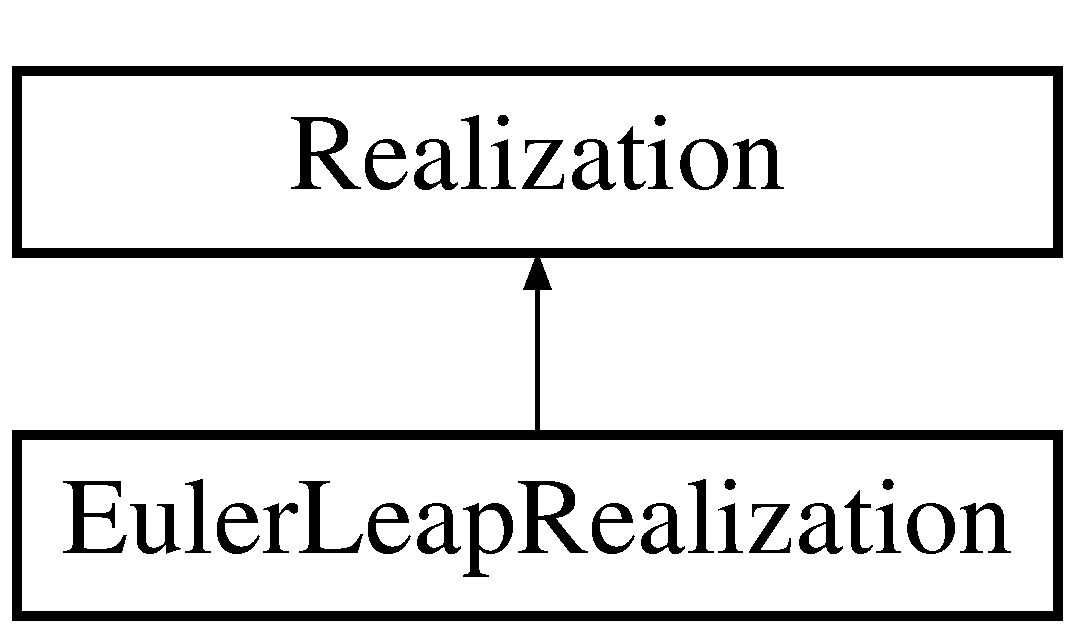
\includegraphics[height=2.000000cm]{class_euler_leap_realization}
\end{center}
\end{figure}
\subsection*{Public Member Functions}
\begin{DoxyCompactItemize}
\item 
\mbox{\Hypertarget{class_euler_leap_realization_ab72bfdc22d6101f2c10227b27a5121f1}\label{class_euler_leap_realization_ab72bfdc22d6101f2c10227b27a5121f1}} 
int {\bfseries step} ()
\end{DoxyCompactItemize}
\subsection*{Additional Inherited Members}


The documentation for this class was generated from the following file\+:\begin{DoxyCompactItemize}
\item 
/\+Users/\+Caleb/\+A\+P\+C524/stoched/src/realization.\+h\end{DoxyCompactItemize}

\hypertarget{class_event}{}\section{Event Class Reference}
\label{class_event}\index{Event@{Event}}


Class \hyperlink{class_event}{Event} holds a user-\/specified event, namely set of functions and associated rate.  




{\ttfamily \#include $<$event.\+h$>$}

\subsection*{Public Member Functions}
\begin{DoxyCompactItemize}
\item 
\hyperlink{class_event_a5a40dd4708297f7031e29b39e039ae10}{Event} ()
\begin{DoxyCompactList}\small\item\em Default constructor for \hyperlink{class_event}{Event}. \end{DoxyCompactList}\item 
\hyperlink{class_event_a7704ec01ce91e673885792054214b3d2}{$\sim$\+Event} ()
\begin{DoxyCompactList}\small\item\em Destructor of \hyperlink{class_event}{Event}. \end{DoxyCompactList}\item 
void \hyperlink{class_event_ad380e41418d2e34b651e052711fefe83}{add\+Function} (string function, string variables)
\begin{DoxyCompactList}\small\item\em Add a function parser to the function array. \end{DoxyCompactList}\item 
double \hyperlink{class_event_a2637844b7f9583caf0f808c898dc2246}{use\+Function} (int i\+Function, double $\ast$args)
\begin{DoxyCompactList}\small\item\em Evaluate function stored at specified spot in the function array. \end{DoxyCompactList}\item 
void \hyperlink{class_event_a993a01984496bc158be92b67422f8655}{set\+Rate} (string function, string variables)
\begin{DoxyCompactList}\small\item\em Set equation for rate\+Function. \end{DoxyCompactList}\item 
double \hyperlink{class_event_a2288e3b3fa19e076e04bba11b88d189a}{get\+Rate} (double $\ast$args)
\begin{DoxyCompactList}\small\item\em Return rate to user based on values of the state array. \end{DoxyCompactList}\item 
int \hyperlink{class_event_a1a0f2e2dc0b203f7be0f1d5b8810c6a2}{get\+Size} ()
\begin{DoxyCompactList}\small\item\em Return size of event, namely number of functions, to user. \end{DoxyCompactList}\item 
double \hyperlink{class_event_afb753b1954fd16e7ba92ae16157f70fd}{get\+Delta\+Var} (int i)
\begin{DoxyCompactList}\small\item\em Return how the ith variable is incremented when the ith equation is called. \end{DoxyCompactList}\item 
void \hyperlink{class_event_a980f39895f2afc1c2273d921d92aeac0}{set\+Delta\+Var} (int i, double val)
\begin{DoxyCompactList}\small\item\em set the amount that the ith function increments the ith variable. This is used by midpoint tau leaping \end{DoxyCompactList}\end{DoxyCompactItemize}
\subsection*{Public Attributes}
\begin{DoxyCompactItemize}
\item 
\mbox{\Hypertarget{class_event_acf8fc6215a0eeaa049e2aca9a347f4b0}\label{class_event_acf8fc6215a0eeaa049e2aca9a347f4b0}} 
string {\bfseries event\+Name}
\end{DoxyCompactItemize}
\subsection*{Private Attributes}
\begin{DoxyCompactItemize}
\item 
\mbox{\Hypertarget{class_event_a77f230a68021756fd1e2d35dcfa534f8}\label{class_event_a77f230a68021756fd1e2d35dcfa534f8}} 
Function\+Parser $\ast$$\ast$ \hyperlink{class_event_a77f230a68021756fd1e2d35dcfa534f8}{function\+Array\+\_\+}
\begin{DoxyCompactList}\small\item\em Array of function parsers. \end{DoxyCompactList}\item 
\mbox{\Hypertarget{class_event_a5a82a70465e39626ad62d1cfe3fc7617}\label{class_event_a5a82a70465e39626ad62d1cfe3fc7617}} 
Function\+Parser \hyperlink{class_event_a5a82a70465e39626ad62d1cfe3fc7617}{rate\+Function}
\begin{DoxyCompactList}\small\item\em Rate specified by an equation. \end{DoxyCompactList}\item 
\mbox{\Hypertarget{class_event_a59244ccd0e0f3654f07715bb3dd6423f}\label{class_event_a59244ccd0e0f3654f07715bb3dd6423f}} 
int \hyperlink{class_event_a59244ccd0e0f3654f07715bb3dd6423f}{eq\+\_\+count\+\_\+}
\begin{DoxyCompactList}\small\item\em Number of function parsers. \end{DoxyCompactList}\item 
\mbox{\Hypertarget{class_event_a869e25f5b77f85372eb0397ea01e25bf}\label{class_event_a869e25f5b77f85372eb0397ea01e25bf}} 
double $\ast$ \hyperlink{class_event_a869e25f5b77f85372eb0397ea01e25bf}{delta\+Var\+\_\+}
\begin{DoxyCompactList}\small\item\em how much each variable in the state changes when its corrsponding function is called. Only used by midpoint tau leaping to calculate approximate continuous time derivative. \end{DoxyCompactList}\end{DoxyCompactItemize}


\subsection{Detailed Description}
Class \hyperlink{class_event}{Event} holds a user-\/specified event, namely set of functions and associated rate. 

\subsection{Constructor \& Destructor Documentation}
\mbox{\Hypertarget{class_event_a5a40dd4708297f7031e29b39e039ae10}\label{class_event_a5a40dd4708297f7031e29b39e039ae10}} 
\index{Event@{Event}!Event@{Event}}
\index{Event@{Event}!Event@{Event}}
\subsubsection{\texorpdfstring{Event()}{Event()}}
{\footnotesize\ttfamily Event\+::\+Event (\begin{DoxyParamCaption}{ }\end{DoxyParamCaption})}



Default constructor for \hyperlink{class_event}{Event}. 


\begin{DoxyParams}{Parameters}
{\em eq\+\_\+count} & is the size of the function array \\
\hline
{\em function\+Array} & contains all user-\/specified Function\+Parsers that govern event \\
\hline
\end{DoxyParams}
\begin{DoxyReturn}{Returns}
nothing 
\end{DoxyReturn}
\mbox{\Hypertarget{class_event_a7704ec01ce91e673885792054214b3d2}\label{class_event_a7704ec01ce91e673885792054214b3d2}} 
\index{Event@{Event}!````~Event@{$\sim$\+Event}}
\index{````~Event@{$\sim$\+Event}!Event@{Event}}
\subsubsection{\texorpdfstring{$\sim$\+Event()}{~Event()}}
{\footnotesize\ttfamily Event\+::$\sim$\+Event (\begin{DoxyParamCaption}{ }\end{DoxyParamCaption})}



Destructor of \hyperlink{class_event}{Event}. 

\begin{DoxyReturn}{Returns}
nothing 
\end{DoxyReturn}


\subsection{Member Function Documentation}
\mbox{\Hypertarget{class_event_ad380e41418d2e34b651e052711fefe83}\label{class_event_ad380e41418d2e34b651e052711fefe83}} 
\index{Event@{Event}!add\+Function@{add\+Function}}
\index{add\+Function@{add\+Function}!Event@{Event}}
\subsubsection{\texorpdfstring{add\+Function()}{addFunction()}}
{\footnotesize\ttfamily void Event\+::add\+Function (\begin{DoxyParamCaption}\item[{string}]{function,  }\item[{string}]{variables }\end{DoxyParamCaption})}



Add a function parser to the function array. 


\begin{DoxyParams}{Parameters}
{\em function} & is a string used to generate a Function\+Parser object \\
\hline
{\em variables} & is a string used to generate a Function\+Parser object \\
\hline
\end{DoxyParams}
\begin{DoxyReturn}{Returns}
void 
\end{DoxyReturn}
\mbox{\Hypertarget{class_event_afb753b1954fd16e7ba92ae16157f70fd}\label{class_event_afb753b1954fd16e7ba92ae16157f70fd}} 
\index{Event@{Event}!get\+Delta\+Var@{get\+Delta\+Var}}
\index{get\+Delta\+Var@{get\+Delta\+Var}!Event@{Event}}
\subsubsection{\texorpdfstring{get\+Delta\+Var()}{getDeltaVar()}}
{\footnotesize\ttfamily double Event\+::get\+Delta\+Var (\begin{DoxyParamCaption}\item[{int}]{i }\end{DoxyParamCaption})}



Return how the ith variable is incremented when the ith equation is called. 


\begin{DoxyParams}{Parameters}
{\em i} & is an int specifying of which variable to find the delta. 0 is the first variable \\
\hline
\end{DoxyParams}
\begin{DoxyReturn}{Returns}
change in value of i when its corresponding equation is called, as a double 
\end{DoxyReturn}
\mbox{\Hypertarget{class_event_a2288e3b3fa19e076e04bba11b88d189a}\label{class_event_a2288e3b3fa19e076e04bba11b88d189a}} 
\index{Event@{Event}!get\+Rate@{get\+Rate}}
\index{get\+Rate@{get\+Rate}!Event@{Event}}
\subsubsection{\texorpdfstring{get\+Rate()}{getRate()}}
{\footnotesize\ttfamily double Event\+::get\+Rate (\begin{DoxyParamCaption}\item[{double $\ast$}]{state\+Array }\end{DoxyParamCaption})}



Return rate to user based on values of the state array. 


\begin{DoxyParams}{Parameters}
{\em state\+Array} & is a double array specifying variable values of function \\
\hline
\end{DoxyParams}
\begin{DoxyReturn}{Returns}
evaluated rate\+Function as a double 
\end{DoxyReturn}
\mbox{\Hypertarget{class_event_a1a0f2e2dc0b203f7be0f1d5b8810c6a2}\label{class_event_a1a0f2e2dc0b203f7be0f1d5b8810c6a2}} 
\index{Event@{Event}!get\+Size@{get\+Size}}
\index{get\+Size@{get\+Size}!Event@{Event}}
\subsubsection{\texorpdfstring{get\+Size()}{getSize()}}
{\footnotesize\ttfamily int Event\+::get\+Size (\begin{DoxyParamCaption}{ }\end{DoxyParamCaption})}



Return size of event, namely number of functions, to user. 

\begin{DoxyReturn}{Returns}
size of event, namely number of functions, as an int 
\end{DoxyReturn}
\mbox{\Hypertarget{class_event_a980f39895f2afc1c2273d921d92aeac0}\label{class_event_a980f39895f2afc1c2273d921d92aeac0}} 
\index{Event@{Event}!set\+Delta\+Var@{set\+Delta\+Var}}
\index{set\+Delta\+Var@{set\+Delta\+Var}!Event@{Event}}
\subsubsection{\texorpdfstring{set\+Delta\+Var()}{setDeltaVar()}}
{\footnotesize\ttfamily void Event\+::set\+Delta\+Var (\begin{DoxyParamCaption}\item[{int}]{i,  }\item[{double}]{val }\end{DoxyParamCaption})}



set the amount that the ith function increments the ith variable. This is used by midpoint tau leaping 


\begin{DoxyParams}{Parameters}
{\em i} & is an int specifying of which variable to set. 0 is the first variable \\
\hline
\end{DoxyParams}
\begin{DoxyReturn}{Returns}
void 
\end{DoxyReturn}
\mbox{\Hypertarget{class_event_a993a01984496bc158be92b67422f8655}\label{class_event_a993a01984496bc158be92b67422f8655}} 
\index{Event@{Event}!set\+Rate@{set\+Rate}}
\index{set\+Rate@{set\+Rate}!Event@{Event}}
\subsubsection{\texorpdfstring{set\+Rate()}{setRate()}}
{\footnotesize\ttfamily void Event\+::set\+Rate (\begin{DoxyParamCaption}\item[{string}]{function,  }\item[{string}]{variables }\end{DoxyParamCaption})}



Set equation for rate\+Function. 


\begin{DoxyParams}{Parameters}
{\em function} & is a string used for parsing rate\+Function \\
\hline
{\em variables} & is a string used for parsing rate\+Function \\
\hline
\end{DoxyParams}
\begin{DoxyReturn}{Returns}
void 
\end{DoxyReturn}
\mbox{\Hypertarget{class_event_a2637844b7f9583caf0f808c898dc2246}\label{class_event_a2637844b7f9583caf0f808c898dc2246}} 
\index{Event@{Event}!use\+Function@{use\+Function}}
\index{use\+Function@{use\+Function}!Event@{Event}}
\subsubsection{\texorpdfstring{use\+Function()}{useFunction()}}
{\footnotesize\ttfamily double Event\+::use\+Function (\begin{DoxyParamCaption}\item[{int}]{i\+Function,  }\item[{double $\ast$}]{state\+Array }\end{DoxyParamCaption})}



Evaluate function stored at specified spot in the function array. 


\begin{DoxyParams}{Parameters}
{\em i\+Function} & is an int that indexes function array \\
\hline
{\em state\+Array} & is a double array specifying variable values of function \\
\hline
\end{DoxyParams}
\begin{DoxyReturn}{Returns}
evaluated function\+Parser as a double 
\end{DoxyReturn}


The documentation for this class was generated from the following files\+:\begin{DoxyCompactItemize}
\item 
/\+Users/dylan/stoched/src/\hyperlink{event_8h}{event.\+h}\item 
/\+Users/dylan/stoched/src/\hyperlink{event_8cc}{event.\+cc}\end{DoxyCompactItemize}

\hypertarget{class_function_parser}{}\section{Function\+Parser Class Reference}
\label{class_function_parser}\index{Function\+Parser@{Function\+Parser}}
Inheritance diagram for Function\+Parser\+:\begin{figure}[H]
\begin{center}
\leavevmode
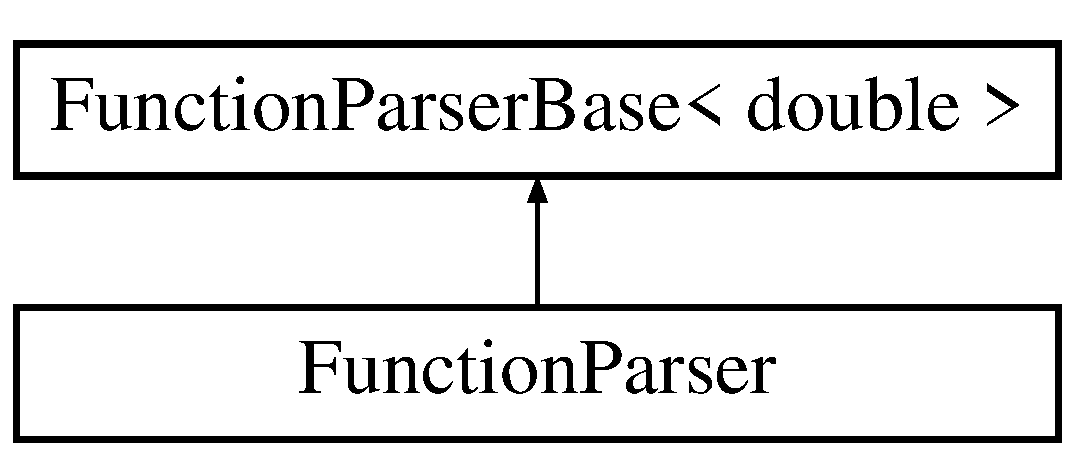
\includegraphics[height=2.000000cm]{class_function_parser}
\end{center}
\end{figure}
\subsection*{Additional Inherited Members}


The documentation for this class was generated from the following file\+:\begin{DoxyCompactItemize}
\item 
/\+Users/\+Caleb/\+A\+P\+C524/stoched/src/fparser/fparser.\+hh\end{DoxyCompactItemize}

\hypertarget{class_function_parser__cd}{}\section{Function\+Parser\+\_\+cd Class Reference}
\label{class_function_parser__cd}\index{Function\+Parser\+\_\+cd@{Function\+Parser\+\_\+cd}}
Inheritance diagram for Function\+Parser\+\_\+cd\+:\begin{figure}[H]
\begin{center}
\leavevmode
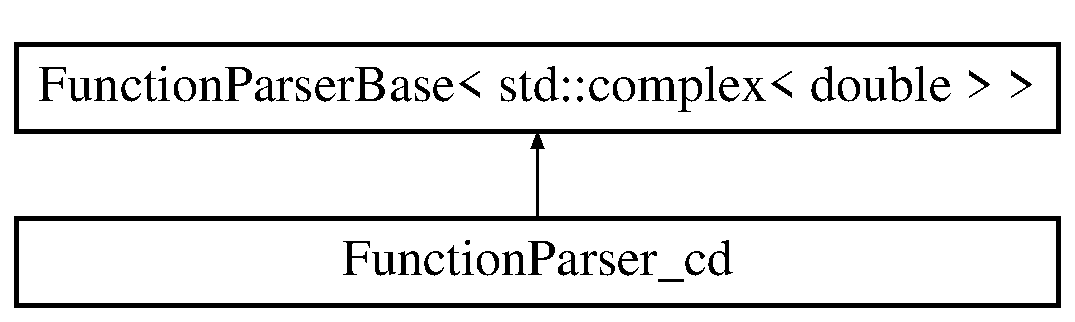
\includegraphics[height=2.000000cm]{class_function_parser__cd}
\end{center}
\end{figure}
\subsection*{Additional Inherited Members}


The documentation for this class was generated from the following file\+:\begin{DoxyCompactItemize}
\item 
/\+Users/\+Caleb/\+A\+P\+C524/stoched/src/fparser/fparser.\+hh\end{DoxyCompactItemize}

\hypertarget{class_function_parser__cf}{}\section{Function\+Parser\+\_\+cf Class Reference}
\label{class_function_parser__cf}\index{Function\+Parser\+\_\+cf@{Function\+Parser\+\_\+cf}}
Inheritance diagram for Function\+Parser\+\_\+cf\+:\begin{figure}[H]
\begin{center}
\leavevmode
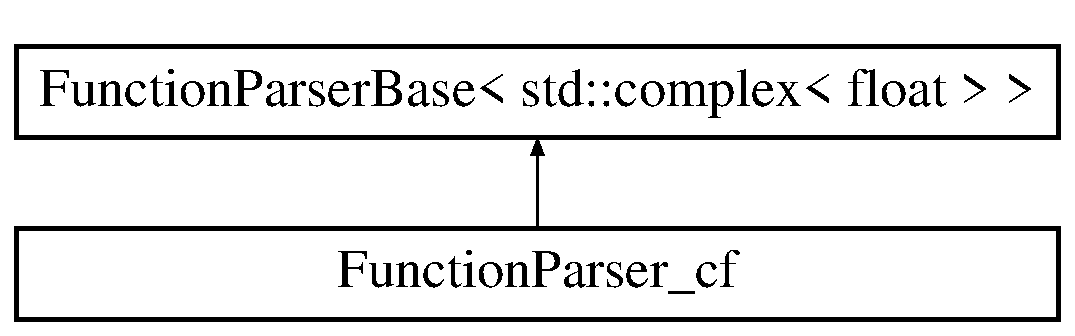
\includegraphics[height=2.000000cm]{class_function_parser__cf}
\end{center}
\end{figure}
\subsection*{Additional Inherited Members}


The documentation for this class was generated from the following file\+:\begin{DoxyCompactItemize}
\item 
/\+Users/\+Caleb/\+A\+P\+C524/stoched/src/fparser/fparser.\+hh\end{DoxyCompactItemize}

\hypertarget{class_function_parser__cld}{}\section{Function\+Parser\+\_\+cld Class Reference}
\label{class_function_parser__cld}\index{Function\+Parser\+\_\+cld@{Function\+Parser\+\_\+cld}}
Inheritance diagram for Function\+Parser\+\_\+cld\+:\begin{figure}[H]
\begin{center}
\leavevmode
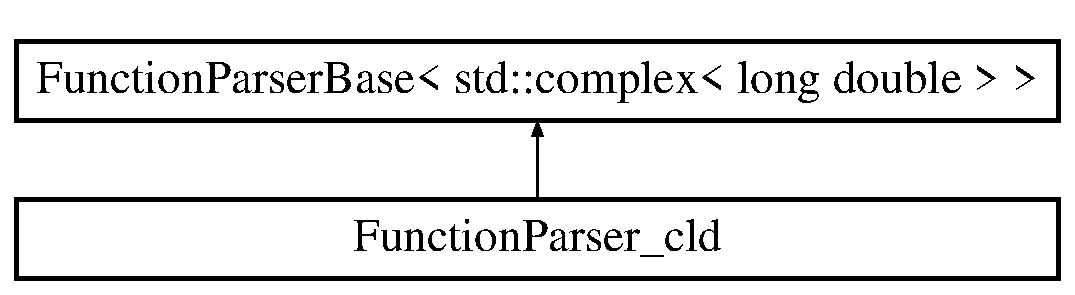
\includegraphics[height=2.000000cm]{class_function_parser__cld}
\end{center}
\end{figure}


The documentation for this class was generated from the following file\+:\begin{DoxyCompactItemize}
\item 
/\+Users/\+Caleb/\+A\+P\+C524/stoched/src/\hyperlink{parser_8y}{parser.\+y}\end{DoxyCompactItemize}

\hypertarget{class_function_parser__f}{}\section{Function\+Parser\+\_\+f Class Reference}
\label{class_function_parser__f}\index{Function\+Parser\+\_\+f@{Function\+Parser\+\_\+f}}
Inheritance diagram for Function\+Parser\+\_\+f\+:\begin{figure}[H]
\begin{center}
\leavevmode
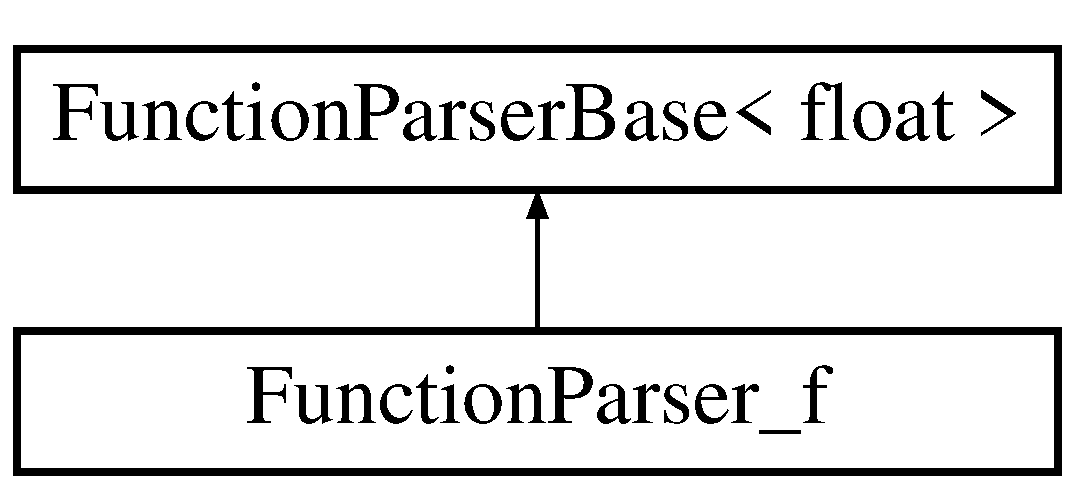
\includegraphics[height=2.000000cm]{class_function_parser__f}
\end{center}
\end{figure}


The documentation for this class was generated from the following file\+:\begin{DoxyCompactItemize}
\item 
/\+Users/\+Caleb/\+A\+P\+C524/stoched/src/\hyperlink{parser_8y}{parser.\+y}\end{DoxyCompactItemize}

\hypertarget{class_function_parser__gmpint}{}\section{Function\+Parser\+\_\+gmpint Class Reference}
\label{class_function_parser__gmpint}\index{Function\+Parser\+\_\+gmpint@{Function\+Parser\+\_\+gmpint}}
Inheritance diagram for Function\+Parser\+\_\+gmpint\+:\begin{figure}[H]
\begin{center}
\leavevmode
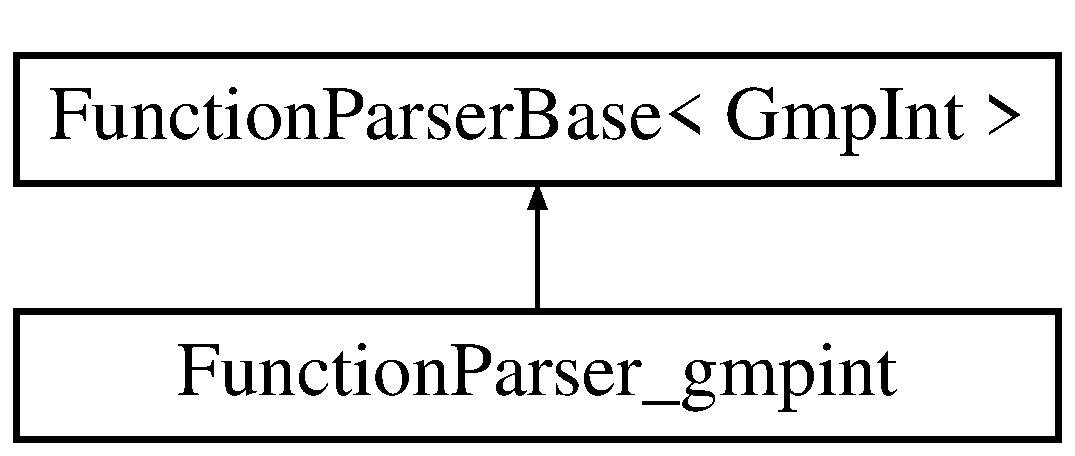
\includegraphics[height=2.000000cm]{class_function_parser__gmpint}
\end{center}
\end{figure}
\subsection*{Additional Inherited Members}


The documentation for this class was generated from the following file\+:\begin{DoxyCompactItemize}
\item 
/\+Users/\+Caleb/\+A\+P\+C524/stoched/src/fparser/fparser\+\_\+gmpint.\+hh\end{DoxyCompactItemize}

\hypertarget{class_function_parser__ld}{}\section{Function\+Parser\+\_\+ld Class Reference}
\label{class_function_parser__ld}\index{Function\+Parser\+\_\+ld@{Function\+Parser\+\_\+ld}}
Inheritance diagram for Function\+Parser\+\_\+ld\+:\begin{figure}[H]
\begin{center}
\leavevmode
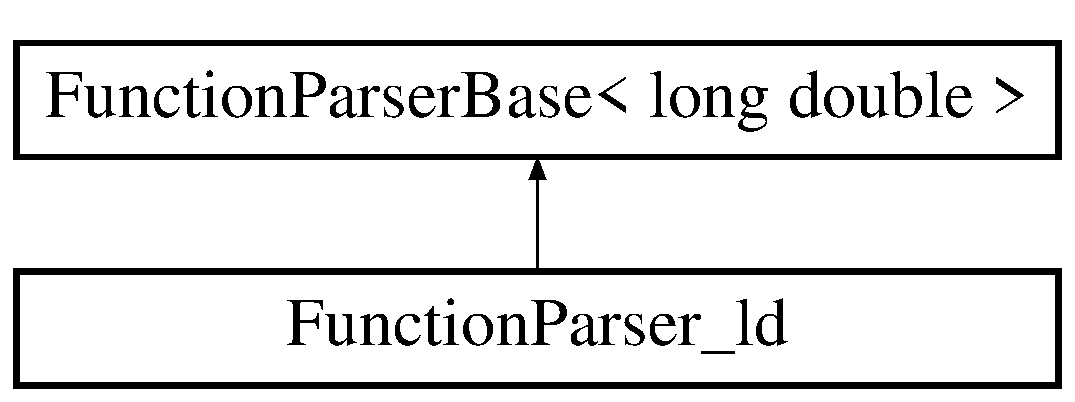
\includegraphics[height=2.000000cm]{class_function_parser__ld}
\end{center}
\end{figure}
\subsection*{Additional Inherited Members}


The documentation for this class was generated from the following file\+:\begin{DoxyCompactItemize}
\item 
/\+Users/\+Caleb/\+A\+P\+C524/stoched/src/fparser/fparser.\+hh\end{DoxyCompactItemize}

\hypertarget{class_function_parser__li}{}\section{Function\+Parser\+\_\+li Class Reference}
\label{class_function_parser__li}\index{Function\+Parser\+\_\+li@{Function\+Parser\+\_\+li}}
Inheritance diagram for Function\+Parser\+\_\+li\+:\begin{figure}[H]
\begin{center}
\leavevmode
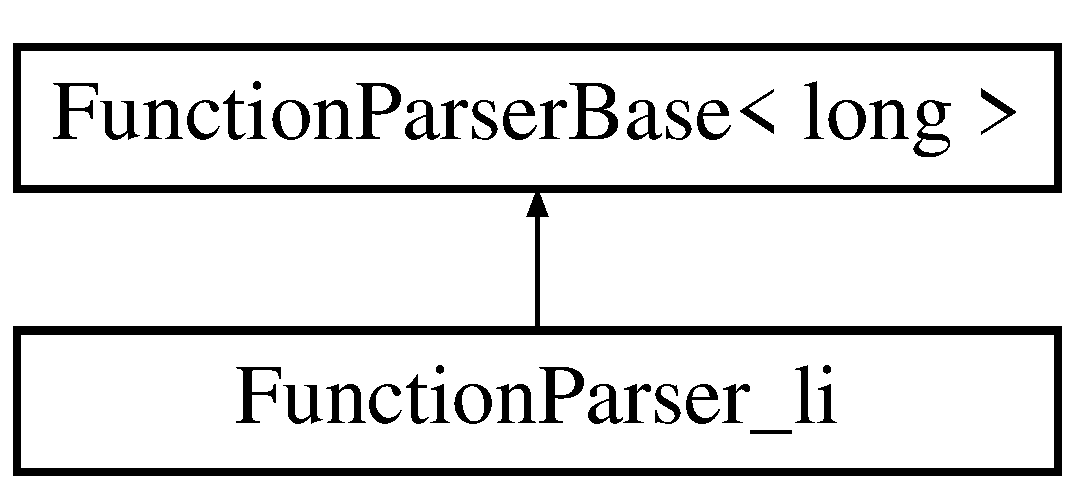
\includegraphics[height=2.000000cm]{class_function_parser__li}
\end{center}
\end{figure}


The documentation for this class was generated from the following file\+:\begin{DoxyCompactItemize}
\item 
/\+Users/\+Caleb/\+A\+P\+C524/stoched/src/\hyperlink{parser_8y}{parser.\+y}\end{DoxyCompactItemize}

\hypertarget{class_function_parser__mpfr}{}\section{Function\+Parser\+\_\+mpfr Class Reference}
\label{class_function_parser__mpfr}\index{Function\+Parser\+\_\+mpfr@{Function\+Parser\+\_\+mpfr}}
Inheritance diagram for Function\+Parser\+\_\+mpfr\+:\begin{figure}[H]
\begin{center}
\leavevmode
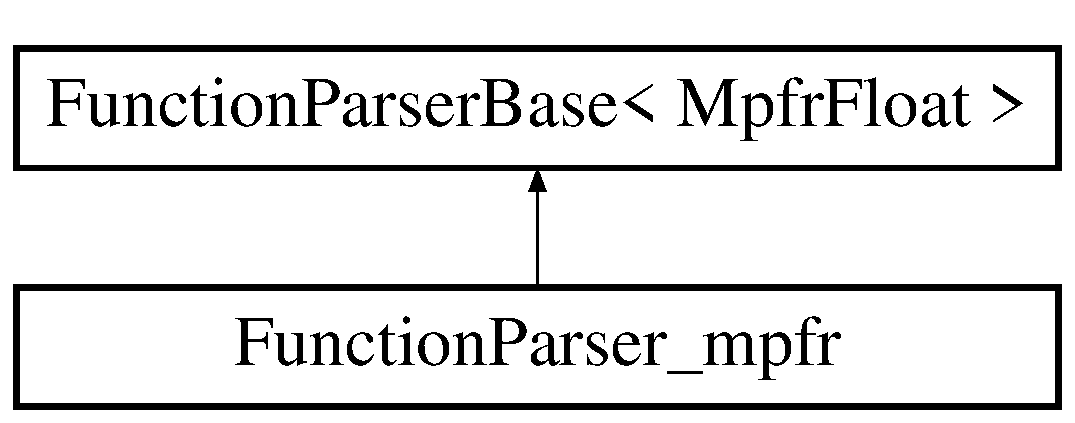
\includegraphics[height=2.000000cm]{class_function_parser__mpfr}
\end{center}
\end{figure}
\subsection*{Additional Inherited Members}


The documentation for this class was generated from the following file\+:\begin{DoxyCompactItemize}
\item 
/\+Users/\+Caleb/\+A\+P\+C524/stoched/src/fparser/fparser\+\_\+mpfr.\+hh\end{DoxyCompactItemize}

\hypertarget{class_function_parser_base}{}\section{Function\+Parser\+Base$<$ Value\+\_\+t $>$ Class Template Reference}
\label{class_function_parser_base}\index{Function\+Parser\+Base$<$ Value\+\_\+t $>$@{Function\+Parser\+Base$<$ Value\+\_\+t $>$}}
\subsection*{Classes}
\begin{DoxyCompactItemize}
\item 
class \hyperlink{class_function_parser_base_1_1_function_wrapper}{Function\+Wrapper}
\end{DoxyCompactItemize}
\subsection*{Public Types}
\begin{DoxyCompactItemize}
\item 
\mbox{\Hypertarget{class_function_parser_base_a1126e1f068b31fb3ea89ffc3918f9aa8}\label{class_function_parser_base_a1126e1f068b31fb3ea89ffc3918f9aa8}} 
enum {\bfseries Parse\+Error\+Type} \{ \newline
{\bfseries S\+Y\+N\+T\+A\+X\+\_\+\+E\+R\+R\+OR} =0, 
{\bfseries M\+I\+S\+M\+\_\+\+P\+A\+R\+E\+N\+TH}, 
{\bfseries M\+I\+S\+S\+I\+N\+G\+\_\+\+P\+A\+R\+E\+N\+TH}, 
{\bfseries E\+M\+P\+T\+Y\+\_\+\+P\+A\+R\+E\+N\+TH}, 
\newline
{\bfseries E\+X\+P\+E\+C\+T\+\_\+\+O\+P\+E\+R\+A\+T\+OR}, 
{\bfseries O\+U\+T\+\_\+\+O\+F\+\_\+\+M\+E\+M\+O\+RY}, 
{\bfseries U\+N\+E\+X\+P\+E\+C\+T\+E\+D\+\_\+\+E\+R\+R\+OR}, 
{\bfseries I\+N\+V\+A\+L\+I\+D\+\_\+\+V\+A\+RS}, 
\newline
{\bfseries I\+L\+L\+\_\+\+P\+A\+R\+A\+M\+S\+\_\+\+A\+M\+O\+U\+NT}, 
{\bfseries P\+R\+E\+M\+A\+T\+U\+R\+E\+\_\+\+E\+OS}, 
{\bfseries E\+X\+P\+E\+C\+T\+\_\+\+P\+A\+R\+E\+N\+T\+H\+\_\+\+F\+U\+NC}, 
{\bfseries U\+N\+K\+N\+O\+W\+N\+\_\+\+I\+D\+E\+N\+T\+I\+F\+I\+ER}, 
\newline
{\bfseries N\+O\+\_\+\+F\+U\+N\+C\+T\+I\+O\+N\+\_\+\+P\+A\+R\+S\+E\+D\+\_\+\+Y\+ET}, 
{\bfseries F\+P\+\_\+\+N\+O\+\_\+\+E\+R\+R\+OR}
 \}
\item 
\mbox{\Hypertarget{class_function_parser_base_a9cc3978ca1d4fca4244b367fc62d4a45}\label{class_function_parser_base_a9cc3978ca1d4fca4244b367fc62d4a45}} 
typedef Value\+\_\+t {\bfseries value\+\_\+type}
\item 
\mbox{\Hypertarget{class_function_parser_base_abf70d4a8970e7174d857c464bf1019a3}\label{class_function_parser_base_abf70d4a8970e7174d857c464bf1019a3}} 
typedef Value\+\_\+t($\ast$ {\bfseries Function\+Ptr}) (const Value\+\_\+t $\ast$)
\end{DoxyCompactItemize}
\subsection*{Public Member Functions}
\begin{DoxyCompactItemize}
\item 
\mbox{\Hypertarget{class_function_parser_base_a11af9197aafaca95459675399a606912}\label{class_function_parser_base_a11af9197aafaca95459675399a606912}} 
int {\bfseries Parse} (const char $\ast$Function, const std\+::string \&Vars, bool use\+Degrees=false)
\item 
\mbox{\Hypertarget{class_function_parser_base_aeee0eb66f38ebc4a7a66fbffac173130}\label{class_function_parser_base_aeee0eb66f38ebc4a7a66fbffac173130}} 
int {\bfseries Parse} (const std\+::string \&Function, const std\+::string \&Vars, bool use\+Degrees=false)
\item 
\mbox{\Hypertarget{class_function_parser_base_ab00b7a9b93a1ff688255a4aaffbb1f19}\label{class_function_parser_base_ab00b7a9b93a1ff688255a4aaffbb1f19}} 
void {\bfseries set\+Delimiter\+Char} (char)
\item 
\mbox{\Hypertarget{class_function_parser_base_a1d81e799766922a212c03021f7366b07}\label{class_function_parser_base_a1d81e799766922a212c03021f7366b07}} 
const char $\ast$ {\bfseries Error\+Msg} () const
\item 
\mbox{\Hypertarget{class_function_parser_base_a6abd7c5d3a1b1ca515d0a35856ee7335}\label{class_function_parser_base_a6abd7c5d3a1b1ca515d0a35856ee7335}} 
Parse\+Error\+Type {\bfseries Get\+Parse\+Error\+Type} () const
\item 
\mbox{\Hypertarget{class_function_parser_base_a2c0d3960126fd7f68541c702dc5e24c5}\label{class_function_parser_base_a2c0d3960126fd7f68541c702dc5e24c5}} 
Value\+\_\+t {\bfseries Eval} (const Value\+\_\+t $\ast$Vars)
\item 
\mbox{\Hypertarget{class_function_parser_base_a8d8d51025306b4db5f734db31a1c0b1c}\label{class_function_parser_base_a8d8d51025306b4db5f734db31a1c0b1c}} 
int {\bfseries Eval\+Error} () const
\item 
\mbox{\Hypertarget{class_function_parser_base_aaab17ce1b0bf03d761c341b255cb5253}\label{class_function_parser_base_aaab17ce1b0bf03d761c341b255cb5253}} 
bool {\bfseries Add\+Constant} (const std\+::string \&name, Value\+\_\+t value)
\item 
\mbox{\Hypertarget{class_function_parser_base_a6d7748f020515ab70b0eb8885595485f}\label{class_function_parser_base_a6d7748f020515ab70b0eb8885595485f}} 
bool {\bfseries Add\+Unit} (const std\+::string \&name, Value\+\_\+t value)
\item 
\mbox{\Hypertarget{class_function_parser_base_a3ce10f1ba66ab8b2682acf0db0b65254}\label{class_function_parser_base_a3ce10f1ba66ab8b2682acf0db0b65254}} 
bool {\bfseries Add\+Function} (const std\+::string \&name, Function\+Ptr, unsigned params\+Amount)
\item 
\mbox{\Hypertarget{class_function_parser_base_aa4925ed099b1708d0690457c414cb386}\label{class_function_parser_base_aa4925ed099b1708d0690457c414cb386}} 
bool {\bfseries Add\+Function} (const std\+::string \&name, \hyperlink{class_function_parser_base}{Function\+Parser\+Base} \&)
\item 
\mbox{\Hypertarget{class_function_parser_base_a2193385ed0850c8124895fa50255bd6b}\label{class_function_parser_base_a2193385ed0850c8124895fa50255bd6b}} 
{\footnotesize template$<$typename Derived\+Wrapper $>$ }\\bool {\bfseries Add\+Function\+Wrapper} (const std\+::string \&name, const Derived\+Wrapper \&, unsigned params\+Amount)
\item 
\mbox{\Hypertarget{class_function_parser_base_a817de51bc1c502df38e14484d4e15140}\label{class_function_parser_base_a817de51bc1c502df38e14484d4e15140}} 
\hyperlink{class_function_parser_base_1_1_function_wrapper}{Function\+Wrapper} $\ast$ {\bfseries Get\+Function\+Wrapper} (const std\+::string \&name)
\item 
\mbox{\Hypertarget{class_function_parser_base_ab8b553d924e2940b8ee3cc00fbd11d10}\label{class_function_parser_base_ab8b553d924e2940b8ee3cc00fbd11d10}} 
bool {\bfseries Remove\+Identifier} (const std\+::string \&name)
\item 
\mbox{\Hypertarget{class_function_parser_base_af25c430d7834d7d1e43b8da5ebaaf382}\label{class_function_parser_base_af25c430d7834d7d1e43b8da5ebaaf382}} 
void {\bfseries Optimize} ()
\item 
\mbox{\Hypertarget{class_function_parser_base_af9911ae70fa2ad7a9b72c83c2b04e371}\label{class_function_parser_base_af9911ae70fa2ad7a9b72c83c2b04e371}} 
int {\bfseries Parse\+And\+Deduce\+Variables} (const std\+::string \&function, int $\ast$amount\+Of\+Variables\+Found=0, bool use\+Degrees=false)
\item 
\mbox{\Hypertarget{class_function_parser_base_a358732851be21c0a4d7391fe121c24e6}\label{class_function_parser_base_a358732851be21c0a4d7391fe121c24e6}} 
int {\bfseries Parse\+And\+Deduce\+Variables} (const std\+::string \&function, std\+::string \&result\+Var\+String, int $\ast$amount\+Of\+Variables\+Found=0, bool use\+Degrees=false)
\item 
\mbox{\Hypertarget{class_function_parser_base_acb8b8d6665d3e3a14e2ffb87b7b92333}\label{class_function_parser_base_acb8b8d6665d3e3a14e2ffb87b7b92333}} 
int {\bfseries Parse\+And\+Deduce\+Variables} (const std\+::string \&function, std\+::vector$<$ std\+::string $>$ \&result\+Vars, bool use\+Degrees=false)
\item 
\mbox{\Hypertarget{class_function_parser_base_a7e61e394eabcf0986e12fa74345b10b9}\label{class_function_parser_base_a7e61e394eabcf0986e12fa74345b10b9}} 
{\bfseries Function\+Parser\+Base} (const \hyperlink{class_function_parser_base}{Function\+Parser\+Base} \&)
\item 
\mbox{\Hypertarget{class_function_parser_base_abf49ad6d28419f75eee77fa5b71defcd}\label{class_function_parser_base_abf49ad6d28419f75eee77fa5b71defcd}} 
\hyperlink{class_function_parser_base}{Function\+Parser\+Base} \& {\bfseries operator=} (const \hyperlink{class_function_parser_base}{Function\+Parser\+Base} \&)
\item 
\mbox{\Hypertarget{class_function_parser_base_a27aa76aa3a554b9210d761c1add2172b}\label{class_function_parser_base_a27aa76aa3a554b9210d761c1add2172b}} 
void {\bfseries Force\+Deep\+Copy} ()
\end{DoxyCompactItemize}
\subsection*{Static Public Member Functions}
\begin{DoxyCompactItemize}
\item 
\mbox{\Hypertarget{class_function_parser_base_a4e45e8962c27cbc0ec62d0a6f9a75cac}\label{class_function_parser_base_a4e45e8962c27cbc0ec62d0a6f9a75cac}} 
static Value\+\_\+t {\bfseries epsilon} ()
\item 
\mbox{\Hypertarget{class_function_parser_base_a694aea0bfb61cd324a753b917f906406}\label{class_function_parser_base_a694aea0bfb61cd324a753b917f906406}} 
static void {\bfseries set\+Epsilon} (Value\+\_\+t)
\end{DoxyCompactItemize}
\subsection*{Protected Member Functions}
\begin{DoxyCompactItemize}
\item 
\mbox{\Hypertarget{class_function_parser_base_a77ea4e232ccb5aca661597f72dc37c84}\label{class_function_parser_base_a77ea4e232ccb5aca661597f72dc37c84}} 
Data $\ast$ {\bfseries get\+Parser\+Data} ()
\end{DoxyCompactItemize}
\subsection*{Static Protected Member Functions}
\begin{DoxyCompactItemize}
\item 
\mbox{\Hypertarget{class_function_parser_base_ad1e1645cc19dff08c61d38680fb18852}\label{class_function_parser_base_ad1e1645cc19dff08c61d38680fb18852}} 
static std\+::pair$<$ const char $\ast$, Value\+\_\+t $>$ {\bfseries Parse\+Literal} (const char $\ast$)
\item 
\mbox{\Hypertarget{class_function_parser_base_a86b9cf2fafc3419ba7964db41fe88e9c}\label{class_function_parser_base_a86b9cf2fafc3419ba7964db41fe88e9c}} 
static unsigned {\bfseries Parse\+Identifier} (const char $\ast$)
\end{DoxyCompactItemize}
\subsection*{Friends}
\begin{DoxyCompactItemize}
\item 
\mbox{\Hypertarget{class_function_parser_base_acf3d682653499dcca599e0d88db26b48}\label{class_function_parser_base_acf3d682653499dcca599e0d88db26b48}} 
class {\bfseries F\+Poptimizer\+\_\+\+Code\+Tree\+::\+Code\+Tree$<$ Value\+\_\+t $>$}
\end{DoxyCompactItemize}


The documentation for this class was generated from the following files\+:\begin{DoxyCompactItemize}
\item 
/\+Users/\+Caleb/\+A\+P\+C524/stoched/src/fparser/fparser.\+hh\item 
/\+Users/\+Caleb/\+A\+P\+C524/stoched/src/fparser/fparser.\+cc\end{DoxyCompactItemize}

\hypertarget{class_function_parser_base_1_1_function_wrapper}{}\section{Function\+Parser\+Base\+:\+:Function\+Wrapper$<$ Value\+\_\+t $>$ Class Template Reference}
\label{class_function_parser_base_1_1_function_wrapper}\index{Function\+Parser\+Base\+::\+Function\+Wrapper$<$ Value\+\_\+t $>$@{Function\+Parser\+Base\+::\+Function\+Wrapper$<$ Value\+\_\+t $>$}}
\subsection*{Public Member Functions}
\begin{DoxyCompactItemize}
\item 
\mbox{\Hypertarget{class_function_parser_base_1_1_function_wrapper_a77a8e2085b1e74a06cdcfc24828a3cce}\label{class_function_parser_base_1_1_function_wrapper_a77a8e2085b1e74a06cdcfc24828a3cce}} 
{\bfseries Function\+Wrapper} (const \hyperlink{class_function_parser_base_1_1_function_wrapper}{Function\+Wrapper} \&)
\item 
\mbox{\Hypertarget{class_function_parser_base_1_1_function_wrapper_addadbef8890ad70616e67ac59ce021a6}\label{class_function_parser_base_1_1_function_wrapper_addadbef8890ad70616e67ac59ce021a6}} 
\hyperlink{class_function_parser_base_1_1_function_wrapper}{Function\+Wrapper} \& {\bfseries operator=} (const \hyperlink{class_function_parser_base_1_1_function_wrapper}{Function\+Wrapper} \&)
\item 
\mbox{\Hypertarget{class_function_parser_base_1_1_function_wrapper_a6528ad7e50401ce8d6c8d5b3c813aa41}\label{class_function_parser_base_1_1_function_wrapper_a6528ad7e50401ce8d6c8d5b3c813aa41}} 
virtual Value\+\_\+t {\bfseries call\+Function} (const Value\+\_\+t $\ast$)=0
\end{DoxyCompactItemize}
\subsection*{Friends}
\begin{DoxyCompactItemize}
\item 
\mbox{\Hypertarget{class_function_parser_base_1_1_function_wrapper_a0c2cfe8c970c6fd489bfe42c8fdf45d6}\label{class_function_parser_base_1_1_function_wrapper_a0c2cfe8c970c6fd489bfe42c8fdf45d6}} 
class {\bfseries Function\+Parser\+Base$<$ Value\+\_\+t $>$}
\end{DoxyCompactItemize}


The documentation for this class was generated from the following file\+:\begin{DoxyCompactItemize}
\item 
/\+Users/\+Caleb/\+A\+P\+C524/stoched/src/\hyperlink{parser_8y}{parser.\+y}\end{DoxyCompactItemize}

\hypertarget{class_gmp_int}{}\section{Gmp\+Int Class Reference}
\label{class_gmp_int}\index{Gmp\+Int@{Gmp\+Int}}
\subsection*{Public Member Functions}
\begin{DoxyCompactItemize}
\item 
\mbox{\Hypertarget{class_gmp_int_aa8353e2c9bef1fc1592409a57934f6a2}\label{class_gmp_int_aa8353e2c9bef1fc1592409a57934f6a2}} 
{\bfseries Gmp\+Int} (long value)
\item 
\mbox{\Hypertarget{class_gmp_int_a5d22f4edbf9bd4e98f061860503ce395}\label{class_gmp_int_a5d22f4edbf9bd4e98f061860503ce395}} 
{\bfseries Gmp\+Int} (unsigned long value)
\item 
\mbox{\Hypertarget{class_gmp_int_a2aed4720584b68430b49a221829b6b77}\label{class_gmp_int_a2aed4720584b68430b49a221829b6b77}} 
{\bfseries Gmp\+Int} (int value)
\item 
\mbox{\Hypertarget{class_gmp_int_a57fe7d80c8af394b9fc6611ca274b6af}\label{class_gmp_int_a57fe7d80c8af394b9fc6611ca274b6af}} 
{\bfseries Gmp\+Int} (double value)
\item 
\mbox{\Hypertarget{class_gmp_int_a1a13efaf5cd6fb68886c1a87579339cc}\label{class_gmp_int_a1a13efaf5cd6fb68886c1a87579339cc}} 
{\bfseries Gmp\+Int} (long double value)
\item 
\mbox{\Hypertarget{class_gmp_int_a4634cc1306298b1b60b973a29c20429c}\label{class_gmp_int_a4634cc1306298b1b60b973a29c20429c}} 
{\bfseries Gmp\+Int} (const \hyperlink{class_gmp_int}{Gmp\+Int} \&)
\item 
\mbox{\Hypertarget{class_gmp_int_aaa554c660aa3bbe03c6f4e0de0b7ffac}\label{class_gmp_int_aaa554c660aa3bbe03c6f4e0de0b7ffac}} 
\hyperlink{class_gmp_int}{Gmp\+Int} \& {\bfseries operator=} (const \hyperlink{class_gmp_int}{Gmp\+Int} \&)
\item 
\mbox{\Hypertarget{class_gmp_int_a43f34a5c89918f74c04990587004ef5e}\label{class_gmp_int_a43f34a5c89918f74c04990587004ef5e}} 
\hyperlink{class_gmp_int}{Gmp\+Int} \& {\bfseries operator=} (signed long value)
\item 
\mbox{\Hypertarget{class_gmp_int_ad971f7fa8334e8802e4e29d3bed73781}\label{class_gmp_int_ad971f7fa8334e8802e4e29d3bed73781}} 
{\footnotesize template$<$typename Mpz\+\_\+t $>$ }\\void {\bfseries get\+\_\+raw\+\_\+mpfr\+\_\+data} (Mpz\+\_\+t \&dest\+\_\+mpz\+\_\+t)
\item 
\mbox{\Hypertarget{class_gmp_int_abd1982de2303e5230bfe87c610cefaa9}\label{class_gmp_int_abd1982de2303e5230bfe87c610cefaa9}} 
const char $\ast$ {\bfseries get\+As\+String} (int base=10) const
\item 
\mbox{\Hypertarget{class_gmp_int_a51a1069df816b6a4a167acbd3b286fda}\label{class_gmp_int_a51a1069df816b6a4a167acbd3b286fda}} 
long {\bfseries to\+Int} () const
\item 
\mbox{\Hypertarget{class_gmp_int_a0720ac71ce8f9042cd50b5ad5d397222}\label{class_gmp_int_a0720ac71ce8f9042cd50b5ad5d397222}} 
\hyperlink{class_gmp_int}{Gmp\+Int} \& {\bfseries operator+=} (const \hyperlink{class_gmp_int}{Gmp\+Int} \&)
\item 
\mbox{\Hypertarget{class_gmp_int_af85c60d76588f7ade3b3356cc5862921}\label{class_gmp_int_af85c60d76588f7ade3b3356cc5862921}} 
\hyperlink{class_gmp_int}{Gmp\+Int} \& {\bfseries operator+=} (long)
\item 
\mbox{\Hypertarget{class_gmp_int_a9c3efd3343771d4142e58e005467b7e1}\label{class_gmp_int_a9c3efd3343771d4142e58e005467b7e1}} 
\hyperlink{class_gmp_int}{Gmp\+Int} \& {\bfseries operator-\/=} (const \hyperlink{class_gmp_int}{Gmp\+Int} \&)
\item 
\mbox{\Hypertarget{class_gmp_int_a2e994af7dec91304557a27b21b36e3df}\label{class_gmp_int_a2e994af7dec91304557a27b21b36e3df}} 
\hyperlink{class_gmp_int}{Gmp\+Int} \& {\bfseries operator-\/=} (long)
\item 
\mbox{\Hypertarget{class_gmp_int_aa3ed85b2f6e11c505fa2a00532fd96fd}\label{class_gmp_int_aa3ed85b2f6e11c505fa2a00532fd96fd}} 
\hyperlink{class_gmp_int}{Gmp\+Int} \& {\bfseries operator$\ast$=} (const \hyperlink{class_gmp_int}{Gmp\+Int} \&)
\item 
\mbox{\Hypertarget{class_gmp_int_a3fc5d0ea3a6ead236fabc7e7d716c692}\label{class_gmp_int_a3fc5d0ea3a6ead236fabc7e7d716c692}} 
\hyperlink{class_gmp_int}{Gmp\+Int} \& {\bfseries operator$\ast$=} (long)
\item 
\mbox{\Hypertarget{class_gmp_int_a17c7bf2f9538ca79edc78fedd635ed68}\label{class_gmp_int_a17c7bf2f9538ca79edc78fedd635ed68}} 
\hyperlink{class_gmp_int}{Gmp\+Int} \& {\bfseries operator/=} (const \hyperlink{class_gmp_int}{Gmp\+Int} \&)
\item 
\mbox{\Hypertarget{class_gmp_int_a9f1d089ade1d26f0bd050dac41a8223b}\label{class_gmp_int_a9f1d089ade1d26f0bd050dac41a8223b}} 
\hyperlink{class_gmp_int}{Gmp\+Int} \& {\bfseries operator/=} (long)
\item 
\mbox{\Hypertarget{class_gmp_int_a1cd7ff6ff736142c3dddef5998a805ad}\label{class_gmp_int_a1cd7ff6ff736142c3dddef5998a805ad}} 
\hyperlink{class_gmp_int}{Gmp\+Int} \& {\bfseries operator\%=} (const \hyperlink{class_gmp_int}{Gmp\+Int} \&)
\item 
\mbox{\Hypertarget{class_gmp_int_a471eb9ea0688a40f13f0616f2d7cb3ca}\label{class_gmp_int_a471eb9ea0688a40f13f0616f2d7cb3ca}} 
\hyperlink{class_gmp_int}{Gmp\+Int} \& {\bfseries operator\%=} (long)
\item 
\mbox{\Hypertarget{class_gmp_int_a843bdf4262c4a51a69f6a2b657c1f358}\label{class_gmp_int_a843bdf4262c4a51a69f6a2b657c1f358}} 
\hyperlink{class_gmp_int}{Gmp\+Int} \& {\bfseries operator$<$$<$=} (unsigned long)
\item 
\mbox{\Hypertarget{class_gmp_int_af675d23e4631edb9f6bb69840b017af8}\label{class_gmp_int_af675d23e4631edb9f6bb69840b017af8}} 
\hyperlink{class_gmp_int}{Gmp\+Int} \& {\bfseries operator$>$$>$=} (unsigned long)
\item 
\mbox{\Hypertarget{class_gmp_int_a6108a1ed85c367f5ab1307be5c02ca75}\label{class_gmp_int_a6108a1ed85c367f5ab1307be5c02ca75}} 
void {\bfseries add\+Product} (const \hyperlink{class_gmp_int}{Gmp\+Int} \&value1, const \hyperlink{class_gmp_int}{Gmp\+Int} \&value2)
\item 
\mbox{\Hypertarget{class_gmp_int_a23d67865bf1d149f868ebf946153dac9}\label{class_gmp_int_a23d67865bf1d149f868ebf946153dac9}} 
void {\bfseries add\+Product} (const \hyperlink{class_gmp_int}{Gmp\+Int} \&value1, unsigned long value2)
\item 
\mbox{\Hypertarget{class_gmp_int_af56e440b21bd5c6bb2980ddda47ba96d}\label{class_gmp_int_af56e440b21bd5c6bb2980ddda47ba96d}} 
void {\bfseries sub\+Product} (const \hyperlink{class_gmp_int}{Gmp\+Int} \&value1, const \hyperlink{class_gmp_int}{Gmp\+Int} \&value2)
\item 
\mbox{\Hypertarget{class_gmp_int_a9ac672feed3c35e1278a124270a75f3b}\label{class_gmp_int_a9ac672feed3c35e1278a124270a75f3b}} 
void {\bfseries sub\+Product} (const \hyperlink{class_gmp_int}{Gmp\+Int} \&value1, unsigned long value2)
\item 
\mbox{\Hypertarget{class_gmp_int_a84208f21b851945f4ab715ba90d10a76}\label{class_gmp_int_a84208f21b851945f4ab715ba90d10a76}} 
void {\bfseries negate} ()
\item 
\mbox{\Hypertarget{class_gmp_int_a817a35ae687775915c608f246d4c3a0f}\label{class_gmp_int_a817a35ae687775915c608f246d4c3a0f}} 
void {\bfseries abs} ()
\item 
\mbox{\Hypertarget{class_gmp_int_ad315055f4f3491a97b1d64dd70329cc6}\label{class_gmp_int_ad315055f4f3491a97b1d64dd70329cc6}} 
\hyperlink{class_gmp_int}{Gmp\+Int} {\bfseries operator+} (const \hyperlink{class_gmp_int}{Gmp\+Int} \&) const
\item 
\mbox{\Hypertarget{class_gmp_int_afe459c1963cc8a9d3f8100fc331e4da5}\label{class_gmp_int_afe459c1963cc8a9d3f8100fc331e4da5}} 
\hyperlink{class_gmp_int}{Gmp\+Int} {\bfseries operator+} (long) const
\item 
\mbox{\Hypertarget{class_gmp_int_ab96f7909f7eb5bf12001be9aea72657f}\label{class_gmp_int_ab96f7909f7eb5bf12001be9aea72657f}} 
\hyperlink{class_gmp_int}{Gmp\+Int} {\bfseries operator-\/} (const \hyperlink{class_gmp_int}{Gmp\+Int} \&) const
\item 
\mbox{\Hypertarget{class_gmp_int_a6c0cf9d7dde28eb302007eae3b013e9b}\label{class_gmp_int_a6c0cf9d7dde28eb302007eae3b013e9b}} 
\hyperlink{class_gmp_int}{Gmp\+Int} {\bfseries operator-\/} (long) const
\item 
\mbox{\Hypertarget{class_gmp_int_af5e0413bc9b89aaf7c4382d2aa08a672}\label{class_gmp_int_af5e0413bc9b89aaf7c4382d2aa08a672}} 
\hyperlink{class_gmp_int}{Gmp\+Int} {\bfseries operator$\ast$} (const \hyperlink{class_gmp_int}{Gmp\+Int} \&) const
\item 
\mbox{\Hypertarget{class_gmp_int_ae9ddbe867e6068be31f7f16370d39a7d}\label{class_gmp_int_ae9ddbe867e6068be31f7f16370d39a7d}} 
\hyperlink{class_gmp_int}{Gmp\+Int} {\bfseries operator$\ast$} (long) const
\item 
\mbox{\Hypertarget{class_gmp_int_aecf1f61a5d8388bb8e78bc525f20102d}\label{class_gmp_int_aecf1f61a5d8388bb8e78bc525f20102d}} 
\hyperlink{class_gmp_int}{Gmp\+Int} {\bfseries operator/} (const \hyperlink{class_gmp_int}{Gmp\+Int} \&) const
\item 
\mbox{\Hypertarget{class_gmp_int_af6cb383f28675a9321a369f129c7461b}\label{class_gmp_int_af6cb383f28675a9321a369f129c7461b}} 
\hyperlink{class_gmp_int}{Gmp\+Int} {\bfseries operator/} (long) const
\item 
\mbox{\Hypertarget{class_gmp_int_a4b4828bf7da7958f0e7349703138d960}\label{class_gmp_int_a4b4828bf7da7958f0e7349703138d960}} 
\hyperlink{class_gmp_int}{Gmp\+Int} {\bfseries operator\%} (const \hyperlink{class_gmp_int}{Gmp\+Int} \&) const
\item 
\mbox{\Hypertarget{class_gmp_int_a00c646809546ce6b15cb1f15b72fbf24}\label{class_gmp_int_a00c646809546ce6b15cb1f15b72fbf24}} 
\hyperlink{class_gmp_int}{Gmp\+Int} {\bfseries operator\%} (long) const
\item 
\mbox{\Hypertarget{class_gmp_int_ac398fe271404fd8cd52da62dcf15c7d9}\label{class_gmp_int_ac398fe271404fd8cd52da62dcf15c7d9}} 
\hyperlink{class_gmp_int}{Gmp\+Int} {\bfseries operator-\/} () const
\item 
\mbox{\Hypertarget{class_gmp_int_af349b7a15ac16a17ab341f6061a910cc}\label{class_gmp_int_af349b7a15ac16a17ab341f6061a910cc}} 
\hyperlink{class_gmp_int}{Gmp\+Int} {\bfseries operator$<$$<$} (unsigned long) const
\item 
\mbox{\Hypertarget{class_gmp_int_a1bc1a03df2dcde64b96aa0cee7bca642}\label{class_gmp_int_a1bc1a03df2dcde64b96aa0cee7bca642}} 
\hyperlink{class_gmp_int}{Gmp\+Int} {\bfseries operator$>$$>$} (unsigned long) const
\item 
\mbox{\Hypertarget{class_gmp_int_a2d8f111fd0545fa966a87052656aad50}\label{class_gmp_int_a2d8f111fd0545fa966a87052656aad50}} 
bool {\bfseries operator$<$} (const \hyperlink{class_gmp_int}{Gmp\+Int} \&) const
\item 
\mbox{\Hypertarget{class_gmp_int_a02c05a80980e0070957ad2afe94271b1}\label{class_gmp_int_a02c05a80980e0070957ad2afe94271b1}} 
bool {\bfseries operator$<$} (long) const
\item 
\mbox{\Hypertarget{class_gmp_int_a9ff21cbfa7e02fd55e5695ae17c9cf1f}\label{class_gmp_int_a9ff21cbfa7e02fd55e5695ae17c9cf1f}} 
bool {\bfseries operator$<$=} (const \hyperlink{class_gmp_int}{Gmp\+Int} \&) const
\item 
\mbox{\Hypertarget{class_gmp_int_a6049c67e480aecf414a28125a9ce3257}\label{class_gmp_int_a6049c67e480aecf414a28125a9ce3257}} 
bool {\bfseries operator$<$=} (long) const
\item 
\mbox{\Hypertarget{class_gmp_int_aef2b82e000e75f177302f3ae7835d9b8}\label{class_gmp_int_aef2b82e000e75f177302f3ae7835d9b8}} 
bool {\bfseries operator$>$} (const \hyperlink{class_gmp_int}{Gmp\+Int} \&) const
\item 
\mbox{\Hypertarget{class_gmp_int_ab1826d58b6369760298d0a35b6757081}\label{class_gmp_int_ab1826d58b6369760298d0a35b6757081}} 
bool {\bfseries operator$>$} (long) const
\item 
\mbox{\Hypertarget{class_gmp_int_a09ecc7acd157cbcd011a83c901051094}\label{class_gmp_int_a09ecc7acd157cbcd011a83c901051094}} 
bool {\bfseries operator$>$=} (const \hyperlink{class_gmp_int}{Gmp\+Int} \&) const
\item 
\mbox{\Hypertarget{class_gmp_int_a5e24d17de3ee02e17c1ce9abcd094d65}\label{class_gmp_int_a5e24d17de3ee02e17c1ce9abcd094d65}} 
bool {\bfseries operator$>$=} (long) const
\item 
\mbox{\Hypertarget{class_gmp_int_aff1fdbede44b450b1ec3c2fe8d17f15b}\label{class_gmp_int_aff1fdbede44b450b1ec3c2fe8d17f15b}} 
bool {\bfseries operator==} (const \hyperlink{class_gmp_int}{Gmp\+Int} \&) const
\item 
\mbox{\Hypertarget{class_gmp_int_a1da3b4c309a1ff532a1e34110311e243}\label{class_gmp_int_a1da3b4c309a1ff532a1e34110311e243}} 
bool {\bfseries operator==} (long) const
\item 
\mbox{\Hypertarget{class_gmp_int_a780da3bcc1e73c203fb95299dda3ee6d}\label{class_gmp_int_a780da3bcc1e73c203fb95299dda3ee6d}} 
bool {\bfseries operator!=} (const \hyperlink{class_gmp_int}{Gmp\+Int} \&) const
\item 
\mbox{\Hypertarget{class_gmp_int_ad6fdbfa0ad3ec0d324b0aa6879b8d6c1}\label{class_gmp_int_ad6fdbfa0ad3ec0d324b0aa6879b8d6c1}} 
bool {\bfseries operator!=} (long) const
\item 
\mbox{\Hypertarget{class_gmp_int_a92a41d198711c2896d2ae7bca42209de}\label{class_gmp_int_a92a41d198711c2896d2ae7bca42209de}} 
void {\bfseries parse\+Value} (const char $\ast$value)
\item 
\mbox{\Hypertarget{class_gmp_int_a79947383c9f80c0867057bbba74cc59a}\label{class_gmp_int_a79947383c9f80c0867057bbba74cc59a}} 
void {\bfseries parse\+Value} (const char $\ast$value, char $\ast$$\ast$endptr)
\item 
\mbox{\Hypertarget{class_gmp_int_ad68c096721eca70fb9ed0f82513008b3}\label{class_gmp_int_ad68c096721eca70fb9ed0f82513008b3}} 
{\footnotesize template$<$$>$ }\\void {\bfseries get\+\_\+raw\+\_\+mpfr\+\_\+data} (mpz\+\_\+t \&dest\+\_\+mpz\+\_\+t)
\end{DoxyCompactItemize}
\subsection*{Static Public Member Functions}
\begin{DoxyCompactItemize}
\item 
\mbox{\Hypertarget{class_gmp_int_a273ae97f8f05b7f9cd01ab5eea9153fc}\label{class_gmp_int_a273ae97f8f05b7f9cd01ab5eea9153fc}} 
static void {\bfseries set\+Default\+Number\+Of\+Bits} (unsigned long)
\item 
\mbox{\Hypertarget{class_gmp_int_a23c5d1a57e1bd9c4415840ed84a3bc6d}\label{class_gmp_int_a23c5d1a57e1bd9c4415840ed84a3bc6d}} 
static unsigned long {\bfseries get\+Default\+Number\+Of\+Bits} ()
\item 
\mbox{\Hypertarget{class_gmp_int_aaeb789d48d137fb5c33bf649187e8b55}\label{class_gmp_int_aaeb789d48d137fb5c33bf649187e8b55}} 
static \hyperlink{class_gmp_int}{Gmp\+Int} {\bfseries abs} (const \hyperlink{class_gmp_int}{Gmp\+Int} \&)
\item 
\mbox{\Hypertarget{class_gmp_int_a5e0da7c2ee351f008be6508fd9011451}\label{class_gmp_int_a5e0da7c2ee351f008be6508fd9011451}} 
static \hyperlink{class_gmp_int}{Gmp\+Int} {\bfseries parse\+String} (const char $\ast$str, char $\ast$$\ast$endptr)
\end{DoxyCompactItemize}
\subsection*{Friends}
\begin{DoxyCompactItemize}
\item 
\mbox{\Hypertarget{class_gmp_int_a117e36d20aff6d0d26e463af039d2bda}\label{class_gmp_int_a117e36d20aff6d0d26e463af039d2bda}} 
\hyperlink{class_gmp_int}{Gmp\+Int} {\bfseries operator+} (long lhs, const \hyperlink{class_gmp_int}{Gmp\+Int} \&rhs)
\item 
\mbox{\Hypertarget{class_gmp_int_a863edd8d21a0737273dbd203169060c0}\label{class_gmp_int_a863edd8d21a0737273dbd203169060c0}} 
\hyperlink{class_gmp_int}{Gmp\+Int} {\bfseries operator-\/} (long lhs, const \hyperlink{class_gmp_int}{Gmp\+Int} \&rhs)
\end{DoxyCompactItemize}


The documentation for this class was generated from the following files\+:\begin{DoxyCompactItemize}
\item 
/\+Users/\+Caleb/\+A\+P\+C524/stoched/src/fparser/mpfr/Gmp\+Int.\+hh\item 
/\+Users/\+Caleb/\+A\+P\+C524/stoched/src/fparser/mpfr/Gmp\+Int.\+cc\end{DoxyCompactItemize}

\hypertarget{struct_gmp_int_1_1_gmp_int_data}{}\section{Gmp\+Int\+:\+:Gmp\+Int\+Data Struct Reference}
\label{struct_gmp_int_1_1_gmp_int_data}\index{Gmp\+Int\+::\+Gmp\+Int\+Data@{Gmp\+Int\+::\+Gmp\+Int\+Data}}
\subsection*{Public Attributes}
\begin{DoxyCompactItemize}
\item 
\mbox{\Hypertarget{struct_gmp_int_1_1_gmp_int_data_ad3f0e1a55b2cf5b0402c155c528cbd53}\label{struct_gmp_int_1_1_gmp_int_data_ad3f0e1a55b2cf5b0402c155c528cbd53}} 
unsigned {\bfseries m\+Ref\+Count}
\item 
\mbox{\Hypertarget{struct_gmp_int_1_1_gmp_int_data_a1f0d48b928272931a8d648aeec256917}\label{struct_gmp_int_1_1_gmp_int_data_a1f0d48b928272931a8d648aeec256917}} 
\hyperlink{struct_gmp_int_1_1_gmp_int_data}{Gmp\+Int\+Data} $\ast$ {\bfseries next\+Free\+Node}
\item 
\mbox{\Hypertarget{struct_gmp_int_1_1_gmp_int_data_a208a3eb034167f1dd8b57aa3c70c96be}\label{struct_gmp_int_1_1_gmp_int_data_a208a3eb034167f1dd8b57aa3c70c96be}} 
mpz\+\_\+t {\bfseries m\+Integer}
\end{DoxyCompactItemize}


The documentation for this struct was generated from the following file\+:\begin{DoxyCompactItemize}
\item 
/\+Users/\+Caleb/\+A\+P\+C524/stoched/src/fparser/mpfr/Gmp\+Int.\+cc\end{DoxyCompactItemize}

\hypertarget{class_gmp_int_1_1_gmp_int_data_container}{}\section{Gmp\+Int\+:\+:Gmp\+Int\+Data\+Container Class Reference}
\label{class_gmp_int_1_1_gmp_int_data_container}\index{Gmp\+Int\+::\+Gmp\+Int\+Data\+Container@{Gmp\+Int\+::\+Gmp\+Int\+Data\+Container}}
\subsection*{Public Member Functions}
\begin{DoxyCompactItemize}
\item 
\mbox{\Hypertarget{class_gmp_int_1_1_gmp_int_data_container_a8624db5a8c851b93a7a17db3390ca2c1}\label{class_gmp_int_1_1_gmp_int_data_container_a8624db5a8c851b93a7a17db3390ca2c1}} 
\hyperlink{struct_gmp_int_1_1_gmp_int_data}{Gmp\+Int\+::\+Gmp\+Int\+Data} $\ast$ {\bfseries allocate\+Gmp\+Int\+Data} (unsigned long number\+Of\+Bits, bool init\+To\+Zero)
\item 
\mbox{\Hypertarget{class_gmp_int_1_1_gmp_int_data_container_ad94f408d14309dd38ebd727f7de6dfb7}\label{class_gmp_int_1_1_gmp_int_data_container_ad94f408d14309dd38ebd727f7de6dfb7}} 
void {\bfseries release\+Gmp\+Int\+Data} (\hyperlink{struct_gmp_int_1_1_gmp_int_data}{Gmp\+Int\+Data} $\ast$data)
\item 
\mbox{\Hypertarget{class_gmp_int_1_1_gmp_int_data_container_a29996fd561aeb8d44daa95508873341f}\label{class_gmp_int_1_1_gmp_int_data_container_a29996fd561aeb8d44daa95508873341f}} 
\hyperlink{struct_gmp_int_1_1_gmp_int_data}{Gmp\+Int\+::\+Gmp\+Int\+Data} $\ast$ {\bfseries const\+\_\+0} ()
\end{DoxyCompactItemize}


The documentation for this class was generated from the following file\+:\begin{DoxyCompactItemize}
\item 
/\+Users/\+Caleb/\+A\+P\+C524/stoched/src/fparser/mpfr/Gmp\+Int.\+cc\end{DoxyCompactItemize}

\hypertarget{class_model}{}\section{Model Class Reference}
\label{class_model}\index{Model@{Model}}


Class M\+O\+D\+EL, which holds user-\/specified models of stochastic systems from which realizations are to be simulated. A model may have variable parameters; each complete set will be stored in an object of class \hyperlink{class_paramset}{Paramset}.  




{\ttfamily \#include $<$model.\+h$>$}

\subsection*{Public Member Functions}
\begin{DoxyCompactItemize}
\item 
\hyperlink{class_model_ae3b375de5f6df4faf74a95d64748e048}{Model} ()
\begin{DoxyCompactList}\small\item\em Default constructor for \hyperlink{class_model}{Model}. \end{DoxyCompactList}\item 
\hyperlink{class_model_ad6ebd2062a0b823db841a0b88baac4c0}{$\sim$\+Model} ()
\begin{DoxyCompactList}\small\item\em Destructor of \hyperlink{class_model}{Model}. \end{DoxyCompactList}\item 
void \hyperlink{class_model_a4743b4f267eeb1a60e21cc2995e1efcd}{add\+Vars} (string vars)
\begin{DoxyCompactList}\small\item\em Add variable list to a \hyperlink{class_model}{Model}. \end{DoxyCompactList}\item 
void \hyperlink{class_model_ab6f784e4ff8cdf3ee5e010ef4dd8d597}{add\+Event} (string function\+Rate)
\begin{DoxyCompactList}\small\item\em Add \hyperlink{class_event}{Event} to \hyperlink{class_model}{Model}\textquotesingle{}s list of Events. \end{DoxyCompactList}\item 
void \hyperlink{class_model_a78d9b07bd5e819215c9aeefabb4cede7}{add\+Event\+Fct} (int i\+Event, string function)
\begin{DoxyCompactList}\small\item\em Add \hyperlink{class_event}{Event} function to specified \hyperlink{class_event}{Event} in \hyperlink{class_model}{Model}. \end{DoxyCompactList}\item 
double \hyperlink{class_model_a774d9fb034f8704a75d7b3568a87a3bc}{use\+Event\+Fct} (int i\+Event, int i\+Function, double $\ast$state\+Array)
\begin{DoxyCompactList}\small\item\em Evaluate given function in specified \hyperlink{class_event}{Event}. \end{DoxyCompactList}\item 
double \hyperlink{class_model_a2909caddddccca90faaae708e68226ad}{get\+Event\+Rate} (int i\+Event, double $\ast$state\+Array)
\begin{DoxyCompactList}\small\item\em Evaluate rate function for a specified \hyperlink{class_event}{Event}. \end{DoxyCompactList}\item 
void \hyperlink{class_model_ad9e7a181a31a2a9fab052d11b1984afd}{update\+State} (int i\+Event, double $\ast$state\+Array)
\begin{DoxyCompactList}\small\item\em Update state array by evaluating all functions of a given \hyperlink{class_event}{Event}. \end{DoxyCompactList}\item 
void \hyperlink{class_model_a3f2fd71261c87162718864d7efc67f2f}{update\+Rates} (double $\ast$state\+Array, double $\ast$rate\+Array)
\begin{DoxyCompactList}\small\item\em Update rate for all Events in \hyperlink{class_model}{Model}\textquotesingle{}s \hyperlink{class_event}{Event} list. \end{DoxyCompactList}\end{DoxyCompactItemize}


\subsection{Detailed Description}
Class M\+O\+D\+EL, which holds user-\/specified models of stochastic systems from which realizations are to be simulated. A model may have variable parameters; each complete set will be stored in an object of class \hyperlink{class_paramset}{Paramset}. 

\subsection{Constructor \& Destructor Documentation}
\mbox{\Hypertarget{class_model_ae3b375de5f6df4faf74a95d64748e048}\label{class_model_ae3b375de5f6df4faf74a95d64748e048}} 
\index{Model@{Model}!Model@{Model}}
\index{Model@{Model}!Model@{Model}}
\subsubsection{\texorpdfstring{Model()}{Model()}}
{\footnotesize\ttfamily Model\+::\+Model (\begin{DoxyParamCaption}{ }\end{DoxyParamCaption})}



Default constructor for \hyperlink{class_model}{Model}. 


\begin{DoxyParams}{Parameters}
{\em none} & \\
\hline
\end{DoxyParams}
\begin{DoxyReturn}{Returns}
nothing 
\end{DoxyReturn}
\mbox{\Hypertarget{class_model_ad6ebd2062a0b823db841a0b88baac4c0}\label{class_model_ad6ebd2062a0b823db841a0b88baac4c0}} 
\index{Model@{Model}!````~Model@{$\sim$\+Model}}
\index{````~Model@{$\sim$\+Model}!Model@{Model}}
\subsubsection{\texorpdfstring{$\sim$\+Model()}{~Model()}}
{\footnotesize\ttfamily Model\+::$\sim$\+Model (\begin{DoxyParamCaption}{ }\end{DoxyParamCaption})}



Destructor of \hyperlink{class_model}{Model}. 


\begin{DoxyParams}{Parameters}
{\em none} & \\
\hline
\end{DoxyParams}
\begin{DoxyReturn}{Returns}
nothing 
\end{DoxyReturn}


\subsection{Member Function Documentation}
\mbox{\Hypertarget{class_model_ab6f784e4ff8cdf3ee5e010ef4dd8d597}\label{class_model_ab6f784e4ff8cdf3ee5e010ef4dd8d597}} 
\index{Model@{Model}!add\+Event@{add\+Event}}
\index{add\+Event@{add\+Event}!Model@{Model}}
\subsubsection{\texorpdfstring{add\+Event()}{addEvent()}}
{\footnotesize\ttfamily void Model\+::add\+Event (\begin{DoxyParamCaption}\item[{string}]{function\+Rate }\end{DoxyParamCaption})}



Add \hyperlink{class_event}{Event} to \hyperlink{class_model}{Model}\textquotesingle{}s list of Events. 


\begin{DoxyParams}{Parameters}
{\em function\+Rate} & is a string that defines an \hyperlink{class_event}{Event}\textquotesingle{}s rate \\
\hline
\end{DoxyParams}
\begin{DoxyReturn}{Returns}
void 
\end{DoxyReturn}
\mbox{\Hypertarget{class_model_a78d9b07bd5e819215c9aeefabb4cede7}\label{class_model_a78d9b07bd5e819215c9aeefabb4cede7}} 
\index{Model@{Model}!add\+Event\+Fct@{add\+Event\+Fct}}
\index{add\+Event\+Fct@{add\+Event\+Fct}!Model@{Model}}
\subsubsection{\texorpdfstring{add\+Event\+Fct()}{addEventFct()}}
{\footnotesize\ttfamily void Model\+::add\+Event\+Fct (\begin{DoxyParamCaption}\item[{int}]{i\+Event,  }\item[{string}]{function }\end{DoxyParamCaption})}



Add \hyperlink{class_event}{Event} function to specified \hyperlink{class_event}{Event} in \hyperlink{class_model}{Model}. 


\begin{DoxyParams}{Parameters}
{\em i\+Event} & is an int that indexes \hyperlink{class_event}{Event} list \\
\hline
{\em function} & is a string that specifies \hyperlink{class_event}{Event} function \\
\hline
\end{DoxyParams}
\begin{DoxyReturn}{Returns}
void 
\end{DoxyReturn}
\mbox{\Hypertarget{class_model_a4743b4f267eeb1a60e21cc2995e1efcd}\label{class_model_a4743b4f267eeb1a60e21cc2995e1efcd}} 
\index{Model@{Model}!add\+Vars@{add\+Vars}}
\index{add\+Vars@{add\+Vars}!Model@{Model}}
\subsubsection{\texorpdfstring{add\+Vars()}{addVars()}}
{\footnotesize\ttfamily void Model\+::add\+Vars (\begin{DoxyParamCaption}\item[{string}]{vars }\end{DoxyParamCaption})}



Add variable list to a \hyperlink{class_model}{Model}. 


\begin{DoxyParams}{Parameters}
{\em vars} & is a string used to set variables associate with a \hyperlink{class_model}{Model} \\
\hline
\end{DoxyParams}
\begin{DoxyReturn}{Returns}
void 
\end{DoxyReturn}
\mbox{\Hypertarget{class_model_a2909caddddccca90faaae708e68226ad}\label{class_model_a2909caddddccca90faaae708e68226ad}} 
\index{Model@{Model}!get\+Event\+Rate@{get\+Event\+Rate}}
\index{get\+Event\+Rate@{get\+Event\+Rate}!Model@{Model}}
\subsubsection{\texorpdfstring{get\+Event\+Rate()}{getEventRate()}}
{\footnotesize\ttfamily double Model\+::get\+Event\+Rate (\begin{DoxyParamCaption}\item[{int}]{i\+Event,  }\item[{double $\ast$}]{state\+Array }\end{DoxyParamCaption})}



Evaluate rate function for a specified \hyperlink{class_event}{Event}. 


\begin{DoxyParams}{Parameters}
{\em i\+Event} & is an int that indexes \hyperlink{class_event}{Event} list \\
\hline
{\em state\+Array} & is a double array specifiying variable values of a function \\
\hline
\end{DoxyParams}
\begin{DoxyReturn}{Returns}
evaluated rate function as a double 
\end{DoxyReturn}
\mbox{\Hypertarget{class_model_a3f2fd71261c87162718864d7efc67f2f}\label{class_model_a3f2fd71261c87162718864d7efc67f2f}} 
\index{Model@{Model}!update\+Rates@{update\+Rates}}
\index{update\+Rates@{update\+Rates}!Model@{Model}}
\subsubsection{\texorpdfstring{update\+Rates()}{updateRates()}}
{\footnotesize\ttfamily void Model\+::update\+Rates (\begin{DoxyParamCaption}\item[{double $\ast$}]{state\+Array,  }\item[{double $\ast$}]{rate\+Array }\end{DoxyParamCaption})}



Update rate for all Events in \hyperlink{class_model}{Model}\textquotesingle{}s \hyperlink{class_event}{Event} list. 


\begin{DoxyParams}{Parameters}
{\em state\+Array} & is a double array specifiying variable values of a function \\
\hline
{\em rate\+Array} & is a double array specifiying variable values of a rate function \\
\hline
\end{DoxyParams}
\begin{DoxyReturn}{Returns}
void 
\end{DoxyReturn}
\mbox{\Hypertarget{class_model_ad9e7a181a31a2a9fab052d11b1984afd}\label{class_model_ad9e7a181a31a2a9fab052d11b1984afd}} 
\index{Model@{Model}!update\+State@{update\+State}}
\index{update\+State@{update\+State}!Model@{Model}}
\subsubsection{\texorpdfstring{update\+State()}{updateState()}}
{\footnotesize\ttfamily void Model\+::update\+State (\begin{DoxyParamCaption}\item[{int}]{i\+Event,  }\item[{double $\ast$}]{state\+Array }\end{DoxyParamCaption})}



Update state array by evaluating all functions of a given \hyperlink{class_event}{Event}. 


\begin{DoxyParams}{Parameters}
{\em i\+Event} & is an int that indexes \hyperlink{class_event}{Event} list \\
\hline
{\em state\+Array} & is a double array specifiying variable values of a function \\
\hline
\end{DoxyParams}
\begin{DoxyReturn}{Returns}
void 
\end{DoxyReturn}
\mbox{\Hypertarget{class_model_a774d9fb034f8704a75d7b3568a87a3bc}\label{class_model_a774d9fb034f8704a75d7b3568a87a3bc}} 
\index{Model@{Model}!use\+Event\+Fct@{use\+Event\+Fct}}
\index{use\+Event\+Fct@{use\+Event\+Fct}!Model@{Model}}
\subsubsection{\texorpdfstring{use\+Event\+Fct()}{useEventFct()}}
{\footnotesize\ttfamily double Model\+::use\+Event\+Fct (\begin{DoxyParamCaption}\item[{int}]{i\+Event,  }\item[{int}]{i\+Function,  }\item[{double $\ast$}]{state\+Array }\end{DoxyParamCaption})}



Evaluate given function in specified \hyperlink{class_event}{Event}. 


\begin{DoxyParams}{Parameters}
{\em i\+Event} & is an int that indexes \hyperlink{class_event}{Event} list \\
\hline
{\em i\+Function} & is an int that indexes an \hyperlink{class_event}{Event}\textquotesingle{}s Function list \\
\hline
{\em state\+Array} & is a double array specifiying variable values of a function \\
\hline
\end{DoxyParams}
\begin{DoxyReturn}{Returns}
evaluated function as a double 
\end{DoxyReturn}


The documentation for this class was generated from the following files\+:\begin{DoxyCompactItemize}
\item 
/\+Users/\+Caleb/\+A\+P\+C524/stoched/src/model.\+h\item 
/\+Users/\+Caleb/\+A\+P\+C524/stoched/src/\hyperlink{model_8cc}{model.\+cc}\end{DoxyCompactItemize}

\hypertarget{class_mpfr_float}{}\section{Mpfr\+Float Class Reference}
\label{class_mpfr_float}\index{Mpfr\+Float@{Mpfr\+Float}}
\subsection*{Public Member Functions}
\begin{DoxyCompactItemize}
\item 
\mbox{\Hypertarget{class_mpfr_float_a984f0977aff05c34e76d3cca363ec6df}\label{class_mpfr_float_a984f0977aff05c34e76d3cca363ec6df}} 
{\bfseries Mpfr\+Float} (double value)
\item 
\mbox{\Hypertarget{class_mpfr_float_a63371995cb8866eb169af680e895ed88}\label{class_mpfr_float_a63371995cb8866eb169af680e895ed88}} 
{\bfseries Mpfr\+Float} (long double value)
\item 
\mbox{\Hypertarget{class_mpfr_float_a69249b46e1caba70b25b4abc1445ba4a}\label{class_mpfr_float_a69249b46e1caba70b25b4abc1445ba4a}} 
{\bfseries Mpfr\+Float} (long value)
\item 
\mbox{\Hypertarget{class_mpfr_float_ad6762394f10890f99bf50b18ec55d880}\label{class_mpfr_float_ad6762394f10890f99bf50b18ec55d880}} 
{\bfseries Mpfr\+Float} (int value)
\item 
\mbox{\Hypertarget{class_mpfr_float_ad90ad26ab3f0a8e135da609af00831c6}\label{class_mpfr_float_ad90ad26ab3f0a8e135da609af00831c6}} 
{\bfseries Mpfr\+Float} (const char $\ast$value, char $\ast$$\ast$endptr)
\item 
\mbox{\Hypertarget{class_mpfr_float_a7bf41a6f17f63864d80819c5248c91c4}\label{class_mpfr_float_a7bf41a6f17f63864d80819c5248c91c4}} 
{\bfseries Mpfr\+Float} (const \hyperlink{class_mpfr_float}{Mpfr\+Float} \&)
\item 
\mbox{\Hypertarget{class_mpfr_float_a09a52144dd7a440a564180879203e25d}\label{class_mpfr_float_a09a52144dd7a440a564180879203e25d}} 
\hyperlink{class_mpfr_float}{Mpfr\+Float} \& {\bfseries operator=} (const \hyperlink{class_mpfr_float}{Mpfr\+Float} \&)
\item 
\mbox{\Hypertarget{class_mpfr_float_aad79999a57423f0f5bccf0881f62a9d5}\label{class_mpfr_float_aad79999a57423f0f5bccf0881f62a9d5}} 
\hyperlink{class_mpfr_float}{Mpfr\+Float} \& {\bfseries operator=} (double value)
\item 
\mbox{\Hypertarget{class_mpfr_float_a64c3e6fc0355299036cae4ba237b4be8}\label{class_mpfr_float_a64c3e6fc0355299036cae4ba237b4be8}} 
\hyperlink{class_mpfr_float}{Mpfr\+Float} \& {\bfseries operator=} (long double value)
\item 
\mbox{\Hypertarget{class_mpfr_float_a1f47b014c02d9c8b379728397f476598}\label{class_mpfr_float_a1f47b014c02d9c8b379728397f476598}} 
\hyperlink{class_mpfr_float}{Mpfr\+Float} \& {\bfseries operator=} (long value)
\item 
\mbox{\Hypertarget{class_mpfr_float_af3f8b35614c1ca05ad2b544f40dcd63f}\label{class_mpfr_float_af3f8b35614c1ca05ad2b544f40dcd63f}} 
\hyperlink{class_mpfr_float}{Mpfr\+Float} \& {\bfseries operator=} (int value)
\item 
\mbox{\Hypertarget{class_mpfr_float_ac1c1e14bd898157a0626b0c18fceed86}\label{class_mpfr_float_ac1c1e14bd898157a0626b0c18fceed86}} 
void {\bfseries parse\+Value} (const char $\ast$value)
\item 
\mbox{\Hypertarget{class_mpfr_float_a6a0991021623ae6843daa977fc1bfd88}\label{class_mpfr_float_a6a0991021623ae6843daa977fc1bfd88}} 
void {\bfseries parse\+Value} (const char $\ast$value, char $\ast$$\ast$endptr)
\item 
\mbox{\Hypertarget{class_mpfr_float_aad6b451d42e2b5c6fc71cb76660c18f6}\label{class_mpfr_float_aad6b451d42e2b5c6fc71cb76660c18f6}} 
{\footnotesize template$<$typename Mpfr\+\_\+t $>$ }\\void {\bfseries get\+\_\+raw\+\_\+mpfr\+\_\+data} (Mpfr\+\_\+t \&dest\+\_\+mpfr\+\_\+t)
\item 
\mbox{\Hypertarget{class_mpfr_float_a87d9334d4840c63a45d163e3b7f24854}\label{class_mpfr_float_a87d9334d4840c63a45d163e3b7f24854}} 
const char $\ast$ {\bfseries get\+As\+String} (unsigned precision) const
\item 
\mbox{\Hypertarget{class_mpfr_float_ae72d4108bd3378ecb75e57e4ca90e6e6}\label{class_mpfr_float_ae72d4108bd3378ecb75e57e4ca90e6e6}} 
bool {\bfseries is\+Integer} () const
\item 
\mbox{\Hypertarget{class_mpfr_float_a28960a654460975191673a8e1b4b031a}\label{class_mpfr_float_a28960a654460975191673a8e1b4b031a}} 
long {\bfseries to\+Int} () const
\item 
\mbox{\Hypertarget{class_mpfr_float_ab751adbadfcb78ed2bbe587948f47ec4}\label{class_mpfr_float_ab751adbadfcb78ed2bbe587948f47ec4}} 
double {\bfseries to\+Double} () const
\item 
\mbox{\Hypertarget{class_mpfr_float_ae300d07da6c4f9aa39c5ad6c75c6fcb2}\label{class_mpfr_float_ae300d07da6c4f9aa39c5ad6c75c6fcb2}} 
\hyperlink{class_mpfr_float}{Mpfr\+Float} \& {\bfseries operator+=} (const \hyperlink{class_mpfr_float}{Mpfr\+Float} \&)
\item 
\mbox{\Hypertarget{class_mpfr_float_a82db05a8be6aedf93a9f5dc87f991245}\label{class_mpfr_float_a82db05a8be6aedf93a9f5dc87f991245}} 
\hyperlink{class_mpfr_float}{Mpfr\+Float} \& {\bfseries operator+=} (double)
\item 
\mbox{\Hypertarget{class_mpfr_float_a072f11c88026d53b5fa53faff0d849f9}\label{class_mpfr_float_a072f11c88026d53b5fa53faff0d849f9}} 
\hyperlink{class_mpfr_float}{Mpfr\+Float} \& {\bfseries operator-\/=} (const \hyperlink{class_mpfr_float}{Mpfr\+Float} \&)
\item 
\mbox{\Hypertarget{class_mpfr_float_a9b0efba241d3f7af25cbb7365ecbfc87}\label{class_mpfr_float_a9b0efba241d3f7af25cbb7365ecbfc87}} 
\hyperlink{class_mpfr_float}{Mpfr\+Float} \& {\bfseries operator-\/=} (double)
\item 
\mbox{\Hypertarget{class_mpfr_float_ad6afb8389c721fc8ad5d195771d8fd7b}\label{class_mpfr_float_ad6afb8389c721fc8ad5d195771d8fd7b}} 
\hyperlink{class_mpfr_float}{Mpfr\+Float} \& {\bfseries operator$\ast$=} (const \hyperlink{class_mpfr_float}{Mpfr\+Float} \&)
\item 
\mbox{\Hypertarget{class_mpfr_float_a81830b08051f8d6079eb8979bdd3c42a}\label{class_mpfr_float_a81830b08051f8d6079eb8979bdd3c42a}} 
\hyperlink{class_mpfr_float}{Mpfr\+Float} \& {\bfseries operator$\ast$=} (double)
\item 
\mbox{\Hypertarget{class_mpfr_float_a08e1a05770675d8b0bcbe294e86d2dff}\label{class_mpfr_float_a08e1a05770675d8b0bcbe294e86d2dff}} 
\hyperlink{class_mpfr_float}{Mpfr\+Float} \& {\bfseries operator/=} (const \hyperlink{class_mpfr_float}{Mpfr\+Float} \&)
\item 
\mbox{\Hypertarget{class_mpfr_float_a3281514648b7f4acd5e8039050847c60}\label{class_mpfr_float_a3281514648b7f4acd5e8039050847c60}} 
\hyperlink{class_mpfr_float}{Mpfr\+Float} \& {\bfseries operator/=} (double)
\item 
\mbox{\Hypertarget{class_mpfr_float_a18c5cd73c8f6d2cfd83fc8b6a53ba330}\label{class_mpfr_float_a18c5cd73c8f6d2cfd83fc8b6a53ba330}} 
\hyperlink{class_mpfr_float}{Mpfr\+Float} \& {\bfseries operator\%=} (const \hyperlink{class_mpfr_float}{Mpfr\+Float} \&)
\item 
\mbox{\Hypertarget{class_mpfr_float_ae638938f0bc54f16891b8c85f91e086e}\label{class_mpfr_float_ae638938f0bc54f16891b8c85f91e086e}} 
void {\bfseries negate} ()
\item 
\mbox{\Hypertarget{class_mpfr_float_a996958ab4054605eed85abafee8ece2d}\label{class_mpfr_float_a996958ab4054605eed85abafee8ece2d}} 
void {\bfseries abs} ()
\item 
\mbox{\Hypertarget{class_mpfr_float_a63225dcc79a58f1e37ac3d4c63831a4e}\label{class_mpfr_float_a63225dcc79a58f1e37ac3d4c63831a4e}} 
\hyperlink{class_mpfr_float}{Mpfr\+Float} {\bfseries operator+} (const \hyperlink{class_mpfr_float}{Mpfr\+Float} \&) const
\item 
\mbox{\Hypertarget{class_mpfr_float_a29fe2d9be874b90ff407e4bbb00b4071}\label{class_mpfr_float_a29fe2d9be874b90ff407e4bbb00b4071}} 
\hyperlink{class_mpfr_float}{Mpfr\+Float} {\bfseries operator+} (double) const
\item 
\mbox{\Hypertarget{class_mpfr_float_ab7e37245e6fbbebfb252f436f5060a3b}\label{class_mpfr_float_ab7e37245e6fbbebfb252f436f5060a3b}} 
\hyperlink{class_mpfr_float}{Mpfr\+Float} {\bfseries operator-\/} (const \hyperlink{class_mpfr_float}{Mpfr\+Float} \&) const
\item 
\mbox{\Hypertarget{class_mpfr_float_a5346ad4c4038a0b071719b6a0e11f959}\label{class_mpfr_float_a5346ad4c4038a0b071719b6a0e11f959}} 
\hyperlink{class_mpfr_float}{Mpfr\+Float} {\bfseries operator-\/} (double) const
\item 
\mbox{\Hypertarget{class_mpfr_float_a9505359f5efd4126937488c1165eb1bd}\label{class_mpfr_float_a9505359f5efd4126937488c1165eb1bd}} 
\hyperlink{class_mpfr_float}{Mpfr\+Float} {\bfseries operator$\ast$} (const \hyperlink{class_mpfr_float}{Mpfr\+Float} \&) const
\item 
\mbox{\Hypertarget{class_mpfr_float_ad67ba7cd219616c35f025bf1f760ecc5}\label{class_mpfr_float_ad67ba7cd219616c35f025bf1f760ecc5}} 
\hyperlink{class_mpfr_float}{Mpfr\+Float} {\bfseries operator$\ast$} (double) const
\item 
\mbox{\Hypertarget{class_mpfr_float_afe0671a46f3c25a0accc570537226995}\label{class_mpfr_float_afe0671a46f3c25a0accc570537226995}} 
\hyperlink{class_mpfr_float}{Mpfr\+Float} {\bfseries operator/} (const \hyperlink{class_mpfr_float}{Mpfr\+Float} \&) const
\item 
\mbox{\Hypertarget{class_mpfr_float_af2ee4339330678bbd62b231b786f4bb6}\label{class_mpfr_float_af2ee4339330678bbd62b231b786f4bb6}} 
\hyperlink{class_mpfr_float}{Mpfr\+Float} {\bfseries operator/} (double) const
\item 
\mbox{\Hypertarget{class_mpfr_float_aa28677307c688c851415eba8781dfdb1}\label{class_mpfr_float_aa28677307c688c851415eba8781dfdb1}} 
\hyperlink{class_mpfr_float}{Mpfr\+Float} {\bfseries operator\%} (const \hyperlink{class_mpfr_float}{Mpfr\+Float} \&) const
\item 
\mbox{\Hypertarget{class_mpfr_float_ad0ee560ba4b18777b512c223ad319c83}\label{class_mpfr_float_ad0ee560ba4b18777b512c223ad319c83}} 
\hyperlink{class_mpfr_float}{Mpfr\+Float} {\bfseries operator-\/} () const
\item 
\mbox{\Hypertarget{class_mpfr_float_adc9033837c117ab9aea2016a5e41257f}\label{class_mpfr_float_adc9033837c117ab9aea2016a5e41257f}} 
bool {\bfseries operator$<$} (const \hyperlink{class_mpfr_float}{Mpfr\+Float} \&) const
\item 
\mbox{\Hypertarget{class_mpfr_float_a3e9f01eef5ed128a38131f75d3b0bd3a}\label{class_mpfr_float_a3e9f01eef5ed128a38131f75d3b0bd3a}} 
bool {\bfseries operator$<$} (double) const
\item 
\mbox{\Hypertarget{class_mpfr_float_a93625bf014bb4cf1c841ab3587d9c1c4}\label{class_mpfr_float_a93625bf014bb4cf1c841ab3587d9c1c4}} 
bool {\bfseries operator$<$=} (const \hyperlink{class_mpfr_float}{Mpfr\+Float} \&) const
\item 
\mbox{\Hypertarget{class_mpfr_float_a92c0d7b6225f45ccee4c8c9797ca70ae}\label{class_mpfr_float_a92c0d7b6225f45ccee4c8c9797ca70ae}} 
bool {\bfseries operator$<$=} (double) const
\item 
\mbox{\Hypertarget{class_mpfr_float_a2fba5909639e2bdeeb7ce5414c05f3f1}\label{class_mpfr_float_a2fba5909639e2bdeeb7ce5414c05f3f1}} 
bool {\bfseries operator$>$} (const \hyperlink{class_mpfr_float}{Mpfr\+Float} \&) const
\item 
\mbox{\Hypertarget{class_mpfr_float_a166f35b91654f9e2431df40b95354060}\label{class_mpfr_float_a166f35b91654f9e2431df40b95354060}} 
bool {\bfseries operator$>$} (double) const
\item 
\mbox{\Hypertarget{class_mpfr_float_a036d170037e1ef0caa63f6deadfac07e}\label{class_mpfr_float_a036d170037e1ef0caa63f6deadfac07e}} 
bool {\bfseries operator$>$=} (const \hyperlink{class_mpfr_float}{Mpfr\+Float} \&) const
\item 
\mbox{\Hypertarget{class_mpfr_float_a63987a7ce1d8ed177cfc83666bcf940f}\label{class_mpfr_float_a63987a7ce1d8ed177cfc83666bcf940f}} 
bool {\bfseries operator$>$=} (double) const
\item 
\mbox{\Hypertarget{class_mpfr_float_a19927b80f5c6e2891d34f9f2db4029de}\label{class_mpfr_float_a19927b80f5c6e2891d34f9f2db4029de}} 
bool {\bfseries operator==} (const \hyperlink{class_mpfr_float}{Mpfr\+Float} \&) const
\item 
\mbox{\Hypertarget{class_mpfr_float_abf46ec39ed5872fd0f7de2ec749c3500}\label{class_mpfr_float_abf46ec39ed5872fd0f7de2ec749c3500}} 
bool {\bfseries operator==} (double) const
\item 
\mbox{\Hypertarget{class_mpfr_float_af4718b3be363b5ef3a9a763ff5b54886}\label{class_mpfr_float_af4718b3be363b5ef3a9a763ff5b54886}} 
bool {\bfseries operator!=} (const \hyperlink{class_mpfr_float}{Mpfr\+Float} \&) const
\item 
\mbox{\Hypertarget{class_mpfr_float_aa335cd3452d48f14dca094be50a725c1}\label{class_mpfr_float_aa335cd3452d48f14dca094be50a725c1}} 
bool {\bfseries operator!=} (double) const
\item 
\mbox{\Hypertarget{class_mpfr_float_a8c44e086174a941b2024e3dafcfd7843}\label{class_mpfr_float_a8c44e086174a941b2024e3dafcfd7843}} 
{\footnotesize template$<$$>$ }\\void {\bfseries get\+\_\+raw\+\_\+mpfr\+\_\+data} (mpfr\+\_\+t \&dest\+\_\+mpfr\+\_\+t)
\end{DoxyCompactItemize}
\subsection*{Static Public Member Functions}
\begin{DoxyCompactItemize}
\item 
\mbox{\Hypertarget{class_mpfr_float_ad78d5a59ad0ba0806b9b6d3447a589c2}\label{class_mpfr_float_ad78d5a59ad0ba0806b9b6d3447a589c2}} 
static void {\bfseries set\+Default\+Mantissa\+Bits} (unsigned long bits)
\item 
\mbox{\Hypertarget{class_mpfr_float_ac6a8002e7d726526076fa421d50104c7}\label{class_mpfr_float_ac6a8002e7d726526076fa421d50104c7}} 
static unsigned long {\bfseries get\+Current\+Default\+Mantissa\+Bits} ()
\item 
\mbox{\Hypertarget{class_mpfr_float_a4f95828fd6e9c53493bd04b018b318b7}\label{class_mpfr_float_a4f95828fd6e9c53493bd04b018b318b7}} 
static \hyperlink{class_mpfr_float}{Mpfr\+Float} {\bfseries log} (const \hyperlink{class_mpfr_float}{Mpfr\+Float} \&)
\item 
\mbox{\Hypertarget{class_mpfr_float_a34baf65e4b91e29f6532b317ec21c93a}\label{class_mpfr_float_a34baf65e4b91e29f6532b317ec21c93a}} 
static \hyperlink{class_mpfr_float}{Mpfr\+Float} {\bfseries log2} (const \hyperlink{class_mpfr_float}{Mpfr\+Float} \&)
\item 
\mbox{\Hypertarget{class_mpfr_float_ac0e0e1e41da174c80e6cf57da7070bb3}\label{class_mpfr_float_ac0e0e1e41da174c80e6cf57da7070bb3}} 
static \hyperlink{class_mpfr_float}{Mpfr\+Float} {\bfseries log10} (const \hyperlink{class_mpfr_float}{Mpfr\+Float} \&)
\item 
\mbox{\Hypertarget{class_mpfr_float_a4811160415c1f52e7d7f44607ff3febd}\label{class_mpfr_float_a4811160415c1f52e7d7f44607ff3febd}} 
static \hyperlink{class_mpfr_float}{Mpfr\+Float} {\bfseries exp} (const \hyperlink{class_mpfr_float}{Mpfr\+Float} \&)
\item 
\mbox{\Hypertarget{class_mpfr_float_a04021ea2a119165ae85288563a2d96a6}\label{class_mpfr_float_a04021ea2a119165ae85288563a2d96a6}} 
static \hyperlink{class_mpfr_float}{Mpfr\+Float} {\bfseries exp2} (const \hyperlink{class_mpfr_float}{Mpfr\+Float} \&)
\item 
\mbox{\Hypertarget{class_mpfr_float_a9d151e2f188c426f63bf6a5e3302932c}\label{class_mpfr_float_a9d151e2f188c426f63bf6a5e3302932c}} 
static \hyperlink{class_mpfr_float}{Mpfr\+Float} {\bfseries exp10} (const \hyperlink{class_mpfr_float}{Mpfr\+Float} \&)
\item 
\mbox{\Hypertarget{class_mpfr_float_a31472a37b4a9f887cf41785da12f87a7}\label{class_mpfr_float_a31472a37b4a9f887cf41785da12f87a7}} 
static \hyperlink{class_mpfr_float}{Mpfr\+Float} {\bfseries cos} (const \hyperlink{class_mpfr_float}{Mpfr\+Float} \&)
\item 
\mbox{\Hypertarget{class_mpfr_float_a7c980d59b703fb365805933289ab1aed}\label{class_mpfr_float_a7c980d59b703fb365805933289ab1aed}} 
static \hyperlink{class_mpfr_float}{Mpfr\+Float} {\bfseries sin} (const \hyperlink{class_mpfr_float}{Mpfr\+Float} \&)
\item 
\mbox{\Hypertarget{class_mpfr_float_a3ebed09f4b532a8c7576bba78287637f}\label{class_mpfr_float_a3ebed09f4b532a8c7576bba78287637f}} 
static \hyperlink{class_mpfr_float}{Mpfr\+Float} {\bfseries tan} (const \hyperlink{class_mpfr_float}{Mpfr\+Float} \&)
\item 
\mbox{\Hypertarget{class_mpfr_float_affa0c0b9e81a97a7943050c573fdd550}\label{class_mpfr_float_affa0c0b9e81a97a7943050c573fdd550}} 
static \hyperlink{class_mpfr_float}{Mpfr\+Float} {\bfseries sec} (const \hyperlink{class_mpfr_float}{Mpfr\+Float} \&)
\item 
\mbox{\Hypertarget{class_mpfr_float_a78df3b7e61935b8af093cdb615d55b89}\label{class_mpfr_float_a78df3b7e61935b8af093cdb615d55b89}} 
static \hyperlink{class_mpfr_float}{Mpfr\+Float} {\bfseries csc} (const \hyperlink{class_mpfr_float}{Mpfr\+Float} \&)
\item 
\mbox{\Hypertarget{class_mpfr_float_a93a126d75c9680f83b3fb1bf129296e9}\label{class_mpfr_float_a93a126d75c9680f83b3fb1bf129296e9}} 
static \hyperlink{class_mpfr_float}{Mpfr\+Float} {\bfseries cot} (const \hyperlink{class_mpfr_float}{Mpfr\+Float} \&)
\item 
\mbox{\Hypertarget{class_mpfr_float_a909ee063cfdbe76bbd4069065f79ae59}\label{class_mpfr_float_a909ee063cfdbe76bbd4069065f79ae59}} 
static void {\bfseries sincos} (const \hyperlink{class_mpfr_float}{Mpfr\+Float} \&, \hyperlink{class_mpfr_float}{Mpfr\+Float} \&sin, \hyperlink{class_mpfr_float}{Mpfr\+Float} \&cos)
\item 
\mbox{\Hypertarget{class_mpfr_float_aab65d26e7eed2e2d767c44d00af30f4d}\label{class_mpfr_float_aab65d26e7eed2e2d767c44d00af30f4d}} 
static \hyperlink{class_mpfr_float}{Mpfr\+Float} {\bfseries acos} (const \hyperlink{class_mpfr_float}{Mpfr\+Float} \&)
\item 
\mbox{\Hypertarget{class_mpfr_float_a1466a8f80f7e1bb6c321f4b8f8c9b47b}\label{class_mpfr_float_a1466a8f80f7e1bb6c321f4b8f8c9b47b}} 
static \hyperlink{class_mpfr_float}{Mpfr\+Float} {\bfseries asin} (const \hyperlink{class_mpfr_float}{Mpfr\+Float} \&)
\item 
\mbox{\Hypertarget{class_mpfr_float_aeb0e653a06e24a90f1b537a5f197924e}\label{class_mpfr_float_aeb0e653a06e24a90f1b537a5f197924e}} 
static \hyperlink{class_mpfr_float}{Mpfr\+Float} {\bfseries atan} (const \hyperlink{class_mpfr_float}{Mpfr\+Float} \&)
\item 
\mbox{\Hypertarget{class_mpfr_float_a75e977a7b3d177945ff6066fd0d5886d}\label{class_mpfr_float_a75e977a7b3d177945ff6066fd0d5886d}} 
static \hyperlink{class_mpfr_float}{Mpfr\+Float} {\bfseries atan2} (const \hyperlink{class_mpfr_float}{Mpfr\+Float} \&, const \hyperlink{class_mpfr_float}{Mpfr\+Float} \&)
\item 
\mbox{\Hypertarget{class_mpfr_float_a804a4854eed469b8295a49a810737ca2}\label{class_mpfr_float_a804a4854eed469b8295a49a810737ca2}} 
static \hyperlink{class_mpfr_float}{Mpfr\+Float} {\bfseries hypot} (const \hyperlink{class_mpfr_float}{Mpfr\+Float} \&, const \hyperlink{class_mpfr_float}{Mpfr\+Float} \&)
\item 
\mbox{\Hypertarget{class_mpfr_float_a923e51dab6f34eea90716225a5e5314c}\label{class_mpfr_float_a923e51dab6f34eea90716225a5e5314c}} 
static \hyperlink{class_mpfr_float}{Mpfr\+Float} {\bfseries cosh} (const \hyperlink{class_mpfr_float}{Mpfr\+Float} \&)
\item 
\mbox{\Hypertarget{class_mpfr_float_a890f6cb75fcbd4b335f52b44de7a97d0}\label{class_mpfr_float_a890f6cb75fcbd4b335f52b44de7a97d0}} 
static \hyperlink{class_mpfr_float}{Mpfr\+Float} {\bfseries sinh} (const \hyperlink{class_mpfr_float}{Mpfr\+Float} \&)
\item 
\mbox{\Hypertarget{class_mpfr_float_add65d7445d86d0968ceea774e16fb3c2}\label{class_mpfr_float_add65d7445d86d0968ceea774e16fb3c2}} 
static \hyperlink{class_mpfr_float}{Mpfr\+Float} {\bfseries tanh} (const \hyperlink{class_mpfr_float}{Mpfr\+Float} \&)
\item 
\mbox{\Hypertarget{class_mpfr_float_a755aff5a0700854e6609b4d6011dd392}\label{class_mpfr_float_a755aff5a0700854e6609b4d6011dd392}} 
static \hyperlink{class_mpfr_float}{Mpfr\+Float} {\bfseries acosh} (const \hyperlink{class_mpfr_float}{Mpfr\+Float} \&)
\item 
\mbox{\Hypertarget{class_mpfr_float_a28580eb116add56d645d0139db189616}\label{class_mpfr_float_a28580eb116add56d645d0139db189616}} 
static \hyperlink{class_mpfr_float}{Mpfr\+Float} {\bfseries asinh} (const \hyperlink{class_mpfr_float}{Mpfr\+Float} \&)
\item 
\mbox{\Hypertarget{class_mpfr_float_ae4d2afb79d933fd346c4dd0b6f76e10b}\label{class_mpfr_float_ae4d2afb79d933fd346c4dd0b6f76e10b}} 
static \hyperlink{class_mpfr_float}{Mpfr\+Float} {\bfseries atanh} (const \hyperlink{class_mpfr_float}{Mpfr\+Float} \&)
\item 
\mbox{\Hypertarget{class_mpfr_float_a2ea23ca0fc60b4318ec32f7d34e8650d}\label{class_mpfr_float_a2ea23ca0fc60b4318ec32f7d34e8650d}} 
static \hyperlink{class_mpfr_float}{Mpfr\+Float} {\bfseries sqrt} (const \hyperlink{class_mpfr_float}{Mpfr\+Float} \&)
\item 
\mbox{\Hypertarget{class_mpfr_float_ac536c18f4eccd3503cefe9f9882783a6}\label{class_mpfr_float_ac536c18f4eccd3503cefe9f9882783a6}} 
static \hyperlink{class_mpfr_float}{Mpfr\+Float} {\bfseries cbrt} (const \hyperlink{class_mpfr_float}{Mpfr\+Float} \&)
\item 
\mbox{\Hypertarget{class_mpfr_float_a077ce8992be43a49b52d6a81921ac26f}\label{class_mpfr_float_a077ce8992be43a49b52d6a81921ac26f}} 
static \hyperlink{class_mpfr_float}{Mpfr\+Float} {\bfseries root} (const \hyperlink{class_mpfr_float}{Mpfr\+Float} \&, unsigned long root)
\item 
\mbox{\Hypertarget{class_mpfr_float_a7e1f2d1da28990f0770a212d7c241afb}\label{class_mpfr_float_a7e1f2d1da28990f0770a212d7c241afb}} 
static \hyperlink{class_mpfr_float}{Mpfr\+Float} {\bfseries pow} (const \hyperlink{class_mpfr_float}{Mpfr\+Float} \&, const \hyperlink{class_mpfr_float}{Mpfr\+Float} \&)
\item 
\mbox{\Hypertarget{class_mpfr_float_a13118af8ab658d366e835e1550e461dd}\label{class_mpfr_float_a13118af8ab658d366e835e1550e461dd}} 
static \hyperlink{class_mpfr_float}{Mpfr\+Float} {\bfseries pow} (const \hyperlink{class_mpfr_float}{Mpfr\+Float} \&, long exponent)
\item 
\mbox{\Hypertarget{class_mpfr_float_a8140e99f8e2a452cb00eb29948fb7609}\label{class_mpfr_float_a8140e99f8e2a452cb00eb29948fb7609}} 
static \hyperlink{class_mpfr_float}{Mpfr\+Float} {\bfseries abs} (const \hyperlink{class_mpfr_float}{Mpfr\+Float} \&)
\item 
\mbox{\Hypertarget{class_mpfr_float_aa33fcf1e5d51e835a42f94c772df6ed8}\label{class_mpfr_float_aa33fcf1e5d51e835a42f94c772df6ed8}} 
static \hyperlink{class_mpfr_float}{Mpfr\+Float} {\bfseries dim} (const \hyperlink{class_mpfr_float}{Mpfr\+Float} \&, const \hyperlink{class_mpfr_float}{Mpfr\+Float} \&)
\item 
\mbox{\Hypertarget{class_mpfr_float_aa9eb65ad04c72f50eade8cc347a49543}\label{class_mpfr_float_aa9eb65ad04c72f50eade8cc347a49543}} 
static \hyperlink{class_mpfr_float}{Mpfr\+Float} {\bfseries round} (const \hyperlink{class_mpfr_float}{Mpfr\+Float} \&)
\item 
\mbox{\Hypertarget{class_mpfr_float_a14b04dcea959cdad4a849e1bddf5bc1d}\label{class_mpfr_float_a14b04dcea959cdad4a849e1bddf5bc1d}} 
static \hyperlink{class_mpfr_float}{Mpfr\+Float} {\bfseries ceil} (const \hyperlink{class_mpfr_float}{Mpfr\+Float} \&)
\item 
\mbox{\Hypertarget{class_mpfr_float_a79b5254d0e97ad5bb6e23342fc98c7d4}\label{class_mpfr_float_a79b5254d0e97ad5bb6e23342fc98c7d4}} 
static \hyperlink{class_mpfr_float}{Mpfr\+Float} {\bfseries floor} (const \hyperlink{class_mpfr_float}{Mpfr\+Float} \&)
\item 
\mbox{\Hypertarget{class_mpfr_float_affbe1e67da1e57258411bdca42e52acc}\label{class_mpfr_float_affbe1e67da1e57258411bdca42e52acc}} 
static \hyperlink{class_mpfr_float}{Mpfr\+Float} {\bfseries trunc} (const \hyperlink{class_mpfr_float}{Mpfr\+Float} \&)
\item 
\mbox{\Hypertarget{class_mpfr_float_a3a9433e0eee8c99d3b3242cec33215be}\label{class_mpfr_float_a3a9433e0eee8c99d3b3242cec33215be}} 
static \hyperlink{class_mpfr_float}{Mpfr\+Float} {\bfseries parse\+String} (const char $\ast$str, char $\ast$$\ast$endptr)
\item 
\mbox{\Hypertarget{class_mpfr_float_a1d7325b12f2746fe76e8a4d071290d32}\label{class_mpfr_float_a1d7325b12f2746fe76e8a4d071290d32}} 
static \hyperlink{class_mpfr_float}{Mpfr\+Float} {\bfseries const\+\_\+pi} ()
\item 
\mbox{\Hypertarget{class_mpfr_float_a8a2736980d7c769f20d465e2bd07b5ad}\label{class_mpfr_float_a8a2736980d7c769f20d465e2bd07b5ad}} 
static \hyperlink{class_mpfr_float}{Mpfr\+Float} {\bfseries const\+\_\+e} ()
\item 
\mbox{\Hypertarget{class_mpfr_float_a4e7ab537851e889df053836a0f638e01}\label{class_mpfr_float_a4e7ab537851e889df053836a0f638e01}} 
static \hyperlink{class_mpfr_float}{Mpfr\+Float} {\bfseries const\+\_\+log2} ()
\item 
\mbox{\Hypertarget{class_mpfr_float_a441261caadbe7f6485080837b5db7397}\label{class_mpfr_float_a441261caadbe7f6485080837b5db7397}} 
static \hyperlink{class_mpfr_float}{Mpfr\+Float} {\bfseries some\+Epsilon} ()
\end{DoxyCompactItemize}
\subsection*{Friends}
\begin{DoxyCompactItemize}
\item 
\mbox{\Hypertarget{class_mpfr_float_a7214b4a42cb61f7e76a24d2dadbf6c50}\label{class_mpfr_float_a7214b4a42cb61f7e76a24d2dadbf6c50}} 
\hyperlink{class_mpfr_float}{Mpfr\+Float} {\bfseries operator+} (double lhs, const \hyperlink{class_mpfr_float}{Mpfr\+Float} \&rhs)
\item 
\mbox{\Hypertarget{class_mpfr_float_a08e7341c10d54073d1e47b0626118776}\label{class_mpfr_float_a08e7341c10d54073d1e47b0626118776}} 
\hyperlink{class_mpfr_float}{Mpfr\+Float} {\bfseries operator-\/} (double lhs, const \hyperlink{class_mpfr_float}{Mpfr\+Float} \&rhs)
\end{DoxyCompactItemize}


The documentation for this class was generated from the following files\+:\begin{DoxyCompactItemize}
\item 
/\+Users/\+Caleb/\+A\+P\+C524/stoched/src/fparser/mpfr/Mpfr\+Float.\+hh\item 
/\+Users/\+Caleb/\+A\+P\+C524/stoched/src/fparser/mpfr/Mpfr\+Float.\+cc\end{DoxyCompactItemize}

\hypertarget{struct_mpfr_float_1_1_mpfr_float_data}{}\section{Mpfr\+Float\+:\+:Mpfr\+Float\+Data Struct Reference}
\label{struct_mpfr_float_1_1_mpfr_float_data}\index{Mpfr\+Float\+::\+Mpfr\+Float\+Data@{Mpfr\+Float\+::\+Mpfr\+Float\+Data}}
\subsection*{Public Attributes}
\begin{DoxyCompactItemize}
\item 
\mbox{\Hypertarget{struct_mpfr_float_1_1_mpfr_float_data_a65c006a9ee36ef49acf88b70a83fc166}\label{struct_mpfr_float_1_1_mpfr_float_data_a65c006a9ee36ef49acf88b70a83fc166}} 
unsigned {\bfseries m\+Ref\+Count}
\item 
\mbox{\Hypertarget{struct_mpfr_float_1_1_mpfr_float_data_afde34bf71430517d44fb89833237fca7}\label{struct_mpfr_float_1_1_mpfr_float_data_afde34bf71430517d44fb89833237fca7}} 
\hyperlink{struct_mpfr_float_1_1_mpfr_float_data}{Mpfr\+Float\+Data} $\ast$ {\bfseries next\+Free\+Node}
\item 
\mbox{\Hypertarget{struct_mpfr_float_1_1_mpfr_float_data_a2f7984309c7bc712a259c9e2bbdc88f6}\label{struct_mpfr_float_1_1_mpfr_float_data_a2f7984309c7bc712a259c9e2bbdc88f6}} 
mpfr\+\_\+t {\bfseries m\+Float}
\end{DoxyCompactItemize}


The documentation for this struct was generated from the following file\+:\begin{DoxyCompactItemize}
\item 
/\+Users/\+Caleb/\+A\+P\+C524/stoched/src/fparser/mpfr/Mpfr\+Float.\+cc\end{DoxyCompactItemize}

\hypertarget{class_mpfr_float_1_1_mpfr_float_data_container}{}\section{Mpfr\+Float\+:\+:Mpfr\+Float\+Data\+Container Class Reference}
\label{class_mpfr_float_1_1_mpfr_float_data_container}\index{Mpfr\+Float\+::\+Mpfr\+Float\+Data\+Container@{Mpfr\+Float\+::\+Mpfr\+Float\+Data\+Container}}
\subsection*{Public Member Functions}
\begin{DoxyCompactItemize}
\item 
\mbox{\Hypertarget{class_mpfr_float_1_1_mpfr_float_data_container_a01979bbcc53978597cb73cc8571b7aca}\label{class_mpfr_float_1_1_mpfr_float_data_container_a01979bbcc53978597cb73cc8571b7aca}} 
\hyperlink{struct_mpfr_float_1_1_mpfr_float_data}{Mpfr\+Float\+Data} $\ast$ {\bfseries allocate\+Mpfr\+Float\+Data} (bool init\+To\+Zero)
\item 
\mbox{\Hypertarget{class_mpfr_float_1_1_mpfr_float_data_container_ac54285f91e4a44f5e515df17d80b5027}\label{class_mpfr_float_1_1_mpfr_float_data_container_ac54285f91e4a44f5e515df17d80b5027}} 
void {\bfseries release\+Mpfr\+Float\+Data} (\hyperlink{struct_mpfr_float_1_1_mpfr_float_data}{Mpfr\+Float\+Data} $\ast$data)
\item 
\mbox{\Hypertarget{class_mpfr_float_1_1_mpfr_float_data_container_a2d6cac131b73904f175cfd6bc9fe60db}\label{class_mpfr_float_1_1_mpfr_float_data_container_a2d6cac131b73904f175cfd6bc9fe60db}} 
void {\bfseries set\+Default\+Precision} (unsigned long bits)
\item 
\mbox{\Hypertarget{class_mpfr_float_1_1_mpfr_float_data_container_a489be7b21d575e1b9047dbd977639b03}\label{class_mpfr_float_1_1_mpfr_float_data_container_a489be7b21d575e1b9047dbd977639b03}} 
unsigned long {\bfseries get\+Default\+Precision} () const
\item 
\mbox{\Hypertarget{class_mpfr_float_1_1_mpfr_float_data_container_a10b2f3355258bf989a9309db255f7d03}\label{class_mpfr_float_1_1_mpfr_float_data_container_a10b2f3355258bf989a9309db255f7d03}} 
\hyperlink{struct_mpfr_float_1_1_mpfr_float_data}{Mpfr\+Float\+Data} $\ast$ {\bfseries const\+\_\+0} ()
\item 
\mbox{\Hypertarget{class_mpfr_float_1_1_mpfr_float_data_container_ade3aa655f2b199aa7aa8029667253c91}\label{class_mpfr_float_1_1_mpfr_float_data_container_ade3aa655f2b199aa7aa8029667253c91}} 
\hyperlink{class_mpfr_float}{Mpfr\+Float} {\bfseries const\+\_\+pi} ()
\item 
\mbox{\Hypertarget{class_mpfr_float_1_1_mpfr_float_data_container_ad47f42390b52eb6f1f668d6d7916b647}\label{class_mpfr_float_1_1_mpfr_float_data_container_ad47f42390b52eb6f1f668d6d7916b647}} 
\hyperlink{class_mpfr_float}{Mpfr\+Float} {\bfseries const\+\_\+e} ()
\item 
\mbox{\Hypertarget{class_mpfr_float_1_1_mpfr_float_data_container_a69abd534e6e19e2ffe3a176ae82f1df4}\label{class_mpfr_float_1_1_mpfr_float_data_container_a69abd534e6e19e2ffe3a176ae82f1df4}} 
\hyperlink{class_mpfr_float}{Mpfr\+Float} {\bfseries const\+\_\+log2} ()
\item 
\mbox{\Hypertarget{class_mpfr_float_1_1_mpfr_float_data_container_a58dde4f07ab5a7598686babddfee3303}\label{class_mpfr_float_1_1_mpfr_float_data_container_a58dde4f07ab5a7598686babddfee3303}} 
\hyperlink{class_mpfr_float}{Mpfr\+Float} {\bfseries const\+\_\+epsilon} ()
\end{DoxyCompactItemize}


The documentation for this class was generated from the following file\+:\begin{DoxyCompactItemize}
\item 
/\+Users/\+Caleb/\+A\+P\+C524/stoched/src/fparser/mpfr/Mpfr\+Float.\+cc\end{DoxyCompactItemize}

\hypertarget{class_paramset}{}\section{Paramset Class Reference}
\label{class_paramset}\index{Paramset@{Paramset}}


Class \hyperlink{class_paramset}{Paramset} holds a particular set of pameters for user requested simulation run(s)  




{\ttfamily \#include $<$paramset.\+h$>$}

\subsection*{Public Member Functions}
\begin{DoxyCompactItemize}
\item 
\hyperlink{class_paramset_aa62d7992b29e74983af7d6026b7111c0}{Paramset} (int \hyperlink{class_paramset_a67376577973f825ba60fc7c319ccc906}{method}, int \hyperlink{class_paramset_aee56c5dcf7d40836397965cdcf392343}{n\+\_\+vars}, double $\ast$\hyperlink{class_paramset_aae7232620d4a9c0bbf30b12c37610c1e}{initial\+\_\+values}, double \hyperlink{class_paramset_a7d82a76c08567e5072aa1b125708c7d8}{t\+\_\+initial}, double \hyperlink{class_paramset_ac88cde461d8dbbd8a7d2636fc45f7119}{t\+\_\+final}, double \hyperlink{class_paramset_a0554913cf803a67bc59ffdee154abc24}{timestep\+\_\+size}, int \hyperlink{class_paramset_a50c0325e75983b66d0825406ec7873ac}{n\+\_\+realizations}, int \hyperlink{class_paramset_afeb86c327cd6966707996019609e6ed1}{max\+\_\+iter}, int \hyperlink{class_paramset_ab8a5866bb87cc2d78a69c47bacaeb06e}{seed})
\begin{DoxyCompactList}\small\item\em Default constructor for \hyperlink{class_paramset}{Paramset}. \end{DoxyCompactList}\item 
\hyperlink{class_paramset_af05c1383de964a28d93e0630d2f4670e}{$\sim$\+Paramset} ()
\begin{DoxyCompactList}\small\item\em Destructor for \hyperlink{class_paramset}{Paramset}. \end{DoxyCompactList}\end{DoxyCompactItemize}
\subsection*{Public Attributes}
\begin{DoxyCompactItemize}
\item 
\mbox{\Hypertarget{class_paramset_a67376577973f825ba60fc7c319ccc906}\label{class_paramset_a67376577973f825ba60fc7c319ccc906}} 
const int \hyperlink{class_paramset_a67376577973f825ba60fc7c319ccc906}{method}
\begin{DoxyCompactList}\small\item\em which algorithm to use for simulation \end{DoxyCompactList}\item 
\mbox{\Hypertarget{class_paramset_aee56c5dcf7d40836397965cdcf392343}\label{class_paramset_aee56c5dcf7d40836397965cdcf392343}} 
const int \hyperlink{class_paramset_aee56c5dcf7d40836397965cdcf392343}{n\+\_\+vars}
\begin{DoxyCompactList}\small\item\em number of initial values/variables \end{DoxyCompactList}\item 
\mbox{\Hypertarget{class_paramset_aae7232620d4a9c0bbf30b12c37610c1e}\label{class_paramset_aae7232620d4a9c0bbf30b12c37610c1e}} 
const double $\ast$ \hyperlink{class_paramset_aae7232620d4a9c0bbf30b12c37610c1e}{initial\+\_\+values}
\begin{DoxyCompactList}\small\item\em initial values for variables \end{DoxyCompactList}\item 
\mbox{\Hypertarget{class_paramset_a7d82a76c08567e5072aa1b125708c7d8}\label{class_paramset_a7d82a76c08567e5072aa1b125708c7d8}} 
const double \hyperlink{class_paramset_a7d82a76c08567e5072aa1b125708c7d8}{t\+\_\+initial}
\begin{DoxyCompactList}\small\item\em initial time for simulation \end{DoxyCompactList}\item 
\mbox{\Hypertarget{class_paramset_ac88cde461d8dbbd8a7d2636fc45f7119}\label{class_paramset_ac88cde461d8dbbd8a7d2636fc45f7119}} 
const double \hyperlink{class_paramset_ac88cde461d8dbbd8a7d2636fc45f7119}{t\+\_\+final}
\begin{DoxyCompactList}\small\item\em final time for simulation \end{DoxyCompactList}\item 
\mbox{\Hypertarget{class_paramset_a0554913cf803a67bc59ffdee154abc24}\label{class_paramset_a0554913cf803a67bc59ffdee154abc24}} 
const double \hyperlink{class_paramset_a0554913cf803a67bc59ffdee154abc24}{timestep\+\_\+size}
\begin{DoxyCompactList}\small\item\em size of timestep for approximate \end{DoxyCompactList}\item 
\mbox{\Hypertarget{class_paramset_a50c0325e75983b66d0825406ec7873ac}\label{class_paramset_a50c0325e75983b66d0825406ec7873ac}} 
int \hyperlink{class_paramset_a50c0325e75983b66d0825406ec7873ac}{n\+\_\+realizations}
\begin{DoxyCompactList}\small\item\em number of realizations to simulate \end{DoxyCompactList}\item 
\mbox{\Hypertarget{class_paramset_afeb86c327cd6966707996019609e6ed1}\label{class_paramset_afeb86c327cd6966707996019609e6ed1}} 
int \hyperlink{class_paramset_afeb86c327cd6966707996019609e6ed1}{max\+\_\+iter}
\begin{DoxyCompactList}\small\item\em max number of iterations to simulate \end{DoxyCompactList}\item 
\mbox{\Hypertarget{class_paramset_ab8a5866bb87cc2d78a69c47bacaeb06e}\label{class_paramset_ab8a5866bb87cc2d78a69c47bacaeb06e}} 
int \hyperlink{class_paramset_ab8a5866bb87cc2d78a69c47bacaeb06e}{seed}
\begin{DoxyCompactList}\small\item\em seed for the random number generator \end{DoxyCompactList}\end{DoxyCompactItemize}


\subsection{Detailed Description}
Class \hyperlink{class_paramset}{Paramset} holds a particular set of pameters for user requested simulation run(s) 

\subsection{Constructor \& Destructor Documentation}
\mbox{\Hypertarget{class_paramset_aa62d7992b29e74983af7d6026b7111c0}\label{class_paramset_aa62d7992b29e74983af7d6026b7111c0}} 
\index{Paramset@{Paramset}!Paramset@{Paramset}}
\index{Paramset@{Paramset}!Paramset@{Paramset}}
\subsubsection{\texorpdfstring{Paramset()}{Paramset()}}
{\footnotesize\ttfamily Paramset\+::\+Paramset (\begin{DoxyParamCaption}\item[{int}]{method,  }\item[{int}]{n\+\_\+vars,  }\item[{double $\ast$}]{initial\+\_\+values,  }\item[{double}]{t\+\_\+initial,  }\item[{double}]{t\+\_\+final,  }\item[{double}]{timestep\+\_\+size,  }\item[{int}]{n\+\_\+realizations,  }\item[{int}]{max\+\_\+iter,  }\item[{int}]{seed }\end{DoxyParamCaption})}



Default constructor for \hyperlink{class_paramset}{Paramset}. 


\begin{DoxyParams}{Parameters}
{\em method} & is an int that specifies algorithm to use for simulation \\
\hline
{\em n\+\_\+vars} & is an int that specifies number of variables \\
\hline
{\em initial\+\_\+values} & is a double array that sets initial values for variables \\
\hline
{\em t\+\_\+initial} & is a double that sets initial time for simulation \\
\hline
{\em t\+\_\+final} & is a double that sets initial time for simulation \\
\hline
{\em timestep\+\_\+size} & is a double representing the size of the timestep for approximate methods \\
\hline
{\em n\+\_\+realizations} & is an int representing number of realizations to simulate \\
\hline
{\em max\+\_\+iter} & is an int and is the maximum number of iterations to simulate \\
\hline
\end{DoxyParams}
\mbox{\Hypertarget{class_paramset_af05c1383de964a28d93e0630d2f4670e}\label{class_paramset_af05c1383de964a28d93e0630d2f4670e}} 
\index{Paramset@{Paramset}!````~Paramset@{$\sim$\+Paramset}}
\index{````~Paramset@{$\sim$\+Paramset}!Paramset@{Paramset}}
\subsubsection{\texorpdfstring{$\sim$\+Paramset()}{~Paramset()}}
{\footnotesize\ttfamily Paramset\+::$\sim$\+Paramset (\begin{DoxyParamCaption}{ }\end{DoxyParamCaption})}



Destructor for \hyperlink{class_paramset}{Paramset}. 

\begin{DoxyReturn}{Returns}
nothing 
\end{DoxyReturn}


The documentation for this class was generated from the following files\+:\begin{DoxyCompactItemize}
\item 
/\+Users/\+Caleb/\+A\+P\+C524/stoched/src/\hyperlink{paramset_8h}{paramset.\+h}\item 
/\+Users/\+Caleb/\+A\+P\+C524/stoched/src/\hyperlink{paramset_8cc}{paramset.\+cc}\end{DoxyCompactItemize}

\hypertarget{class_realization}{}\section{Realization Class Reference}
\label{class_realization}\index{Realization@{Realization}}


Class \hyperlink{class_realization}{Realization} holds realizations of a \hyperlink{class_model}{Model} (state array, propensities, waiting times, etc.)  




{\ttfamily \#include $<$realization.\+h$>$}

Inheritance diagram for Realization\+:\begin{figure}[H]
\begin{center}
\leavevmode
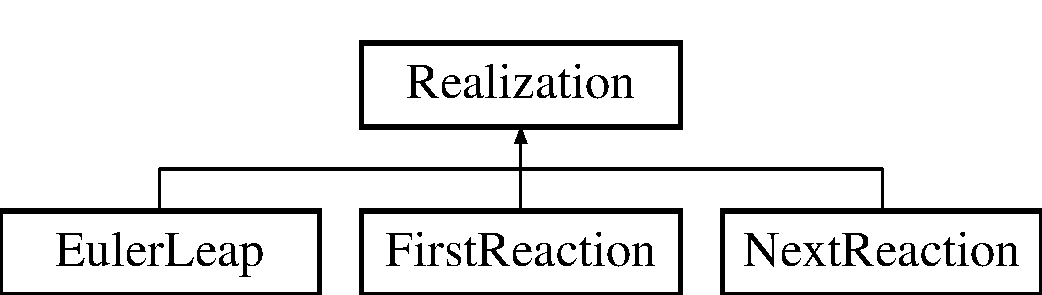
\includegraphics[height=2.000000cm]{class_realization}
\end{center}
\end{figure}
\subsection*{Public Member Functions}
\begin{DoxyCompactItemize}
\item 
\hyperlink{class_realization_af4cfb6f2221bef9ba5ad09564796677f}{Realization} (\hyperlink{class_model}{Model} $\ast$\hyperlink{class_realization_a47ec1d062b8caee874b08c1a17d6aeeb}{the\+\_\+model}, const \hyperlink{class_paramset}{Paramset} \&\hyperlink{class_realization_a119bb29de88929bc51bc1b329473a94b}{the\+\_\+paramset}, \hyperlink{classrng}{rng} $\ast$\hyperlink{class_realization_ac8d358d929afae90cf5790675b6744f9}{the\+\_\+rng}, int \hyperlink{class_realization_ad9951a0829e68e12fcb3817735bb5097}{n\+\_\+vars}, int \hyperlink{class_realization_afb711282bef806fc0020f91252d1df2c}{n\+\_\+events})
\begin{DoxyCompactList}\small\item\em Default constructor for \hyperlink{class_realization}{Realization}. \end{DoxyCompactList}\item 
virtual \hyperlink{class_realization_a040c39b39c5057c668bd264b4329f2b4}{$\sim$\+Realization} ()
\begin{DoxyCompactList}\small\item\em Destructor of \hyperlink{class_realization}{Realization}. \end{DoxyCompactList}\item 
int \hyperlink{class_realization_a4e21bc7355e33c17d1401736b3c62413}{simulate} (std\+::ofstream \&myfile)
\begin{DoxyCompactList}\small\item\em Simulates the realization from t\+\_\+inital to t\+\_\+final. \end{DoxyCompactList}\item 
\mbox{\Hypertarget{class_realization_a9949217117927b149850288f3b74c9ef}\label{class_realization_a9949217117927b149850288f3b74c9ef}} 
virtual int \hyperlink{class_realization_a9949217117927b149850288f3b74c9ef}{step} ()=0
\begin{DoxyCompactList}\small\item\em takes one simulation step according to the chosen algorithm \end{DoxyCompactList}\item 
bool \hyperlink{class_realization_a48953442ebf235cd1e02731c7419f65f}{rates\+\_\+are\+\_\+zero} ()
\begin{DoxyCompactList}\small\item\em checks whether all rates are zero \end{DoxyCompactList}\item 
int \hyperlink{class_realization_ab7ef90279eef4bf11261084f541c7bb0}{output\+\_\+state} (std\+::ofstream \&myfile)
\begin{DoxyCompactList}\small\item\em Prints the current state of the simulation. \end{DoxyCompactList}\item 
virtual int \hyperlink{class_realization_a391a89af7574a9053f53f8a299c2cc70}{set\+\_\+to\+\_\+initial\+\_\+state} ()
\begin{DoxyCompactList}\small\item\em Sets state\+\_\+array and state\+\_\+time to their user-\/specified initial values. \end{DoxyCompactList}\end{DoxyCompactItemize}
\subsection*{Public Attributes}
\begin{DoxyCompactItemize}
\item 
\mbox{\Hypertarget{class_realization_a47ec1d062b8caee874b08c1a17d6aeeb}\label{class_realization_a47ec1d062b8caee874b08c1a17d6aeeb}} 
\hyperlink{class_model}{Model} $\ast$ \hyperlink{class_realization_a47ec1d062b8caee874b08c1a17d6aeeb}{the\+\_\+model}
\begin{DoxyCompactList}\small\item\em the\+\_\+model is a \hyperlink{class_model}{Model} instance \end{DoxyCompactList}\item 
\mbox{\Hypertarget{class_realization_a119bb29de88929bc51bc1b329473a94b}\label{class_realization_a119bb29de88929bc51bc1b329473a94b}} 
const \hyperlink{class_paramset}{Paramset} \hyperlink{class_realization_a119bb29de88929bc51bc1b329473a94b}{the\+\_\+paramset}
\begin{DoxyCompactList}\small\item\em the\+\_\+paramset is a \hyperlink{class_paramset}{Paramset} instance \end{DoxyCompactList}\item 
\mbox{\Hypertarget{class_realization_ac8d358d929afae90cf5790675b6744f9}\label{class_realization_ac8d358d929afae90cf5790675b6744f9}} 
\hyperlink{classrng}{rng} $\ast$ \hyperlink{class_realization_ac8d358d929afae90cf5790675b6744f9}{the\+\_\+rng}
\begin{DoxyCompactList}\small\item\em the\+\_\+rng is an random number generator \end{DoxyCompactList}\item 
\mbox{\Hypertarget{class_realization_ad9951a0829e68e12fcb3817735bb5097}\label{class_realization_ad9951a0829e68e12fcb3817735bb5097}} 
const int \hyperlink{class_realization_ad9951a0829e68e12fcb3817735bb5097}{n\+\_\+vars}
\begin{DoxyCompactList}\small\item\em n\+\_\+vars is an int specifying number of variables \end{DoxyCompactList}\item 
\mbox{\Hypertarget{class_realization_afb711282bef806fc0020f91252d1df2c}\label{class_realization_afb711282bef806fc0020f91252d1df2c}} 
const int \hyperlink{class_realization_afb711282bef806fc0020f91252d1df2c}{n\+\_\+events}
\begin{DoxyCompactList}\small\item\em n\+\_\+events is an int specifying number of events \end{DoxyCompactList}\item 
\mbox{\Hypertarget{class_realization_a126f89978f0407873473222171333ee1}\label{class_realization_a126f89978f0407873473222171333ee1}} 
double $\ast$ \hyperlink{class_realization_a126f89978f0407873473222171333ee1}{state\+\_\+array}
\begin{DoxyCompactList}\small\item\em state\+\_\+array is a double array specifiying variable values of a function \end{DoxyCompactList}\item 
\mbox{\Hypertarget{class_realization_a9c52d8c6aa0ad99dbbec1e98302db7d8}\label{class_realization_a9c52d8c6aa0ad99dbbec1e98302db7d8}} 
double $\ast$ \hyperlink{class_realization_a9c52d8c6aa0ad99dbbec1e98302db7d8}{rates}
\begin{DoxyCompactList}\small\item\em rates is a double array specifying variable values of a rate function \end{DoxyCompactList}\item 
\mbox{\Hypertarget{class_realization_a7c4def45c4833072317517b71e723793}\label{class_realization_a7c4def45c4833072317517b71e723793}} 
double \hyperlink{class_realization_a7c4def45c4833072317517b71e723793}{state\+\_\+time}
\begin{DoxyCompactList}\small\item\em state\+\_\+time is a double that tracks state progress \end{DoxyCompactList}\end{DoxyCompactItemize}


\subsection{Detailed Description}
Class \hyperlink{class_realization}{Realization} holds realizations of a \hyperlink{class_model}{Model} (state array, propensities, waiting times, etc.) 

\subsection{Constructor \& Destructor Documentation}
\mbox{\Hypertarget{class_realization_af4cfb6f2221bef9ba5ad09564796677f}\label{class_realization_af4cfb6f2221bef9ba5ad09564796677f}} 
\index{Realization@{Realization}!Realization@{Realization}}
\index{Realization@{Realization}!Realization@{Realization}}
\subsubsection{\texorpdfstring{Realization()}{Realization()}}
{\footnotesize\ttfamily Realization\+::\+Realization (\begin{DoxyParamCaption}\item[{\hyperlink{class_model}{Model} $\ast$}]{the\+\_\+model,  }\item[{const \hyperlink{class_paramset}{Paramset} \&}]{the\+\_\+paramset,  }\item[{\hyperlink{classrng}{rng} $\ast$}]{the\+\_\+rng,  }\item[{int}]{n\+\_\+vars,  }\item[{int}]{n\+\_\+events }\end{DoxyParamCaption})}



Default constructor for \hyperlink{class_realization}{Realization}. 


\begin{DoxyParams}{Parameters}
{\em the\+\_\+model} & is a \hyperlink{class_model}{Model} object \\
\hline
{\em the\+\_\+paramset} & is a \hyperlink{class_paramset}{Paramset} object \\
\hline
{\em the\+\_\+rng} & is a random number generator \\
\hline
{\em n\+\_\+vars} & is an int specifying variable count \\
\hline
{\em n\+\_\+events} & is an int specifying event count\\
\hline
\end{DoxyParams}
\begin{DoxyReturn}{Returns}
nothing 
\end{DoxyReturn}
\mbox{\Hypertarget{class_realization_a040c39b39c5057c668bd264b4329f2b4}\label{class_realization_a040c39b39c5057c668bd264b4329f2b4}} 
\index{Realization@{Realization}!````~Realization@{$\sim$\+Realization}}
\index{````~Realization@{$\sim$\+Realization}!Realization@{Realization}}
\subsubsection{\texorpdfstring{$\sim$\+Realization()}{~Realization()}}
{\footnotesize\ttfamily Realization\+::$\sim$\+Realization (\begin{DoxyParamCaption}{ }\end{DoxyParamCaption})\hspace{0.3cm}{\ttfamily [virtual]}}



Destructor of \hyperlink{class_realization}{Realization}. 

\begin{DoxyReturn}{Returns}
nothing 
\end{DoxyReturn}


\subsection{Member Function Documentation}
\mbox{\Hypertarget{class_realization_ab7ef90279eef4bf11261084f541c7bb0}\label{class_realization_ab7ef90279eef4bf11261084f541c7bb0}} 
\index{Realization@{Realization}!output\+\_\+state@{output\+\_\+state}}
\index{output\+\_\+state@{output\+\_\+state}!Realization@{Realization}}
\subsubsection{\texorpdfstring{output\+\_\+state()}{output\_state()}}
{\footnotesize\ttfamily int Realization\+::output\+\_\+state (\begin{DoxyParamCaption}\item[{std\+::ofstream \&}]{myfile }\end{DoxyParamCaption})}



Prints the current state of the simulation. 

\begin{DoxyReturn}{Returns}
int 
\end{DoxyReturn}
\mbox{\Hypertarget{class_realization_a48953442ebf235cd1e02731c7419f65f}\label{class_realization_a48953442ebf235cd1e02731c7419f65f}} 
\index{Realization@{Realization}!rates\+\_\+are\+\_\+zero@{rates\+\_\+are\+\_\+zero}}
\index{rates\+\_\+are\+\_\+zero@{rates\+\_\+are\+\_\+zero}!Realization@{Realization}}
\subsubsection{\texorpdfstring{rates\+\_\+are\+\_\+zero()}{rates\_are\_zero()}}
{\footnotesize\ttfamily bool Realization\+::rates\+\_\+are\+\_\+zero (\begin{DoxyParamCaption}{ }\end{DoxyParamCaption})}



checks whether all rates are zero 

\begin{DoxyReturn}{Returns}
bool 
\end{DoxyReturn}
\mbox{\Hypertarget{class_realization_a391a89af7574a9053f53f8a299c2cc70}\label{class_realization_a391a89af7574a9053f53f8a299c2cc70}} 
\index{Realization@{Realization}!set\+\_\+to\+\_\+initial\+\_\+state@{set\+\_\+to\+\_\+initial\+\_\+state}}
\index{set\+\_\+to\+\_\+initial\+\_\+state@{set\+\_\+to\+\_\+initial\+\_\+state}!Realization@{Realization}}
\subsubsection{\texorpdfstring{set\+\_\+to\+\_\+initial\+\_\+state()}{set\_to\_initial\_state()}}
{\footnotesize\ttfamily int Realization\+::set\+\_\+to\+\_\+initial\+\_\+state (\begin{DoxyParamCaption}{ }\end{DoxyParamCaption})\hspace{0.3cm}{\ttfamily [virtual]}}



Sets state\+\_\+array and state\+\_\+time to their user-\/specified initial values. 

\begin{DoxyReturn}{Returns}
int 
\end{DoxyReturn}


Reimplemented in \hyperlink{class_euler_leap_a1a13929ea1ebf40e7357439968828f4b}{Euler\+Leap}, \hyperlink{class_midpoint_leap_a177682cf5042407ccee1a443e8920896}{Midpoint\+Leap}, and \hyperlink{class_next_reaction_a0cc63c4ec9fe3f338472fff302f6d746}{Next\+Reaction}.

\mbox{\Hypertarget{class_realization_a4e21bc7355e33c17d1401736b3c62413}\label{class_realization_a4e21bc7355e33c17d1401736b3c62413}} 
\index{Realization@{Realization}!simulate@{simulate}}
\index{simulate@{simulate}!Realization@{Realization}}
\subsubsection{\texorpdfstring{simulate()}{simulate()}}
{\footnotesize\ttfamily int Realization\+::simulate (\begin{DoxyParamCaption}\item[{std\+::ofstream \&}]{myfile }\end{DoxyParamCaption})}



Simulates the realization from t\+\_\+inital to t\+\_\+final. 

\begin{DoxyReturn}{Returns}
int 
\end{DoxyReturn}


The documentation for this class was generated from the following files\+:\begin{DoxyCompactItemize}
\item 
/\+Users/\+Caleb/\+A\+P\+C524/stoched/src/\hyperlink{realization_8h}{realization.\+h}\item 
/\+Users/\+Caleb/\+A\+P\+C524/stoched/src/\hyperlink{realization_8cc}{realization.\+cc}\end{DoxyCompactItemize}

\hypertarget{classx_q}{}\section{xQ Class Reference}
\label{classx_q}\index{xQ@{xQ}}


The documentation for this class was generated from the following file\+:\begin{DoxyCompactItemize}
\item 
/\+Users/\+Caleb/\+A\+P\+C524/stoched/src/fparser/fpoptimizer.\+cc\end{DoxyCompactItemize}

\hypertarget{structyy__buffer__state}{}\section{yy\+\_\+buffer\+\_\+state Struct Reference}
\label{structyy__buffer__state}\index{yy\+\_\+buffer\+\_\+state@{yy\+\_\+buffer\+\_\+state}}
\subsection*{Public Attributes}
\begin{DoxyCompactItemize}
\item 
\mbox{\Hypertarget{structyy__buffer__state_a4843d1422e3276b636d475a3095bd948}\label{structyy__buffer__state_a4843d1422e3276b636d475a3095bd948}} 
F\+I\+LE $\ast$ {\bfseries yy\+\_\+input\+\_\+file}
\item 
\mbox{\Hypertarget{structyy__buffer__state_ad7b8df8d8a4688e57b0b8d3ca75adc85}\label{structyy__buffer__state_ad7b8df8d8a4688e57b0b8d3ca75adc85}} 
char $\ast$ {\bfseries yy\+\_\+ch\+\_\+buf}
\item 
\mbox{\Hypertarget{structyy__buffer__state_a58aa927f098b99d99e75da80f9b681ef}\label{structyy__buffer__state_a58aa927f098b99d99e75da80f9b681ef}} 
char $\ast$ {\bfseries yy\+\_\+buf\+\_\+pos}
\item 
\mbox{\Hypertarget{structyy__buffer__state_a48302f5f3477a9c78bbddf56d356ef54}\label{structyy__buffer__state_a48302f5f3477a9c78bbddf56d356ef54}} 
yy\+\_\+size\+\_\+t {\bfseries yy\+\_\+buf\+\_\+size}
\item 
\mbox{\Hypertarget{structyy__buffer__state_afcc44872643f513e79b43c2b1f334a67}\label{structyy__buffer__state_afcc44872643f513e79b43c2b1f334a67}} 
yy\+\_\+size\+\_\+t {\bfseries yy\+\_\+n\+\_\+chars}
\item 
\mbox{\Hypertarget{structyy__buffer__state_a80ce2431c70dc4f89ced487f18449465}\label{structyy__buffer__state_a80ce2431c70dc4f89ced487f18449465}} 
int {\bfseries yy\+\_\+is\+\_\+our\+\_\+buffer}
\item 
\mbox{\Hypertarget{structyy__buffer__state_abf5c70eea75581b58c0ee7bd31b14490}\label{structyy__buffer__state_abf5c70eea75581b58c0ee7bd31b14490}} 
int {\bfseries yy\+\_\+is\+\_\+interactive}
\item 
\mbox{\Hypertarget{structyy__buffer__state_a9d60c60af6e1a6f69de16871fd64f85f}\label{structyy__buffer__state_a9d60c60af6e1a6f69de16871fd64f85f}} 
int {\bfseries yy\+\_\+at\+\_\+bol}
\item 
int \hyperlink{structyy__buffer__state_a818e94bc9c766e683c60df1e9fd01199}{yy\+\_\+bs\+\_\+lineno}
\item 
int \hyperlink{structyy__buffer__state_a10c4fcd8be759e6bf11e6d3e8cdb0307}{yy\+\_\+bs\+\_\+column}
\item 
\mbox{\Hypertarget{structyy__buffer__state_a63d2afbb1d79a3fc63df9e12626f827d}\label{structyy__buffer__state_a63d2afbb1d79a3fc63df9e12626f827d}} 
int {\bfseries yy\+\_\+fill\+\_\+buffer}
\item 
\mbox{\Hypertarget{structyy__buffer__state_a70fd925d37a2f0454fbd0def675d106c}\label{structyy__buffer__state_a70fd925d37a2f0454fbd0def675d106c}} 
int {\bfseries yy\+\_\+buffer\+\_\+status}
\end{DoxyCompactItemize}


\subsection{Member Data Documentation}
\mbox{\Hypertarget{structyy__buffer__state_a10c4fcd8be759e6bf11e6d3e8cdb0307}\label{structyy__buffer__state_a10c4fcd8be759e6bf11e6d3e8cdb0307}} 
\index{yy\+\_\+buffer\+\_\+state@{yy\+\_\+buffer\+\_\+state}!yy\+\_\+bs\+\_\+column@{yy\+\_\+bs\+\_\+column}}
\index{yy\+\_\+bs\+\_\+column@{yy\+\_\+bs\+\_\+column}!yy\+\_\+buffer\+\_\+state@{yy\+\_\+buffer\+\_\+state}}
\subsubsection{\texorpdfstring{yy\+\_\+bs\+\_\+column}{yy\_bs\_column}}
{\footnotesize\ttfamily int yy\+\_\+buffer\+\_\+state\+::yy\+\_\+bs\+\_\+column}

The column count. \mbox{\Hypertarget{structyy__buffer__state_a818e94bc9c766e683c60df1e9fd01199}\label{structyy__buffer__state_a818e94bc9c766e683c60df1e9fd01199}} 
\index{yy\+\_\+buffer\+\_\+state@{yy\+\_\+buffer\+\_\+state}!yy\+\_\+bs\+\_\+lineno@{yy\+\_\+bs\+\_\+lineno}}
\index{yy\+\_\+bs\+\_\+lineno@{yy\+\_\+bs\+\_\+lineno}!yy\+\_\+buffer\+\_\+state@{yy\+\_\+buffer\+\_\+state}}
\subsubsection{\texorpdfstring{yy\+\_\+bs\+\_\+lineno}{yy\_bs\_lineno}}
{\footnotesize\ttfamily int yy\+\_\+buffer\+\_\+state\+::yy\+\_\+bs\+\_\+lineno}

The line count. 

The documentation for this struct was generated from the following file\+:\begin{DoxyCompactItemize}
\item 
/\+Users/\+Caleb/\+A\+P\+C524/stoched/src/lex.\+yy.\+c\end{DoxyCompactItemize}

\hypertarget{structyy__trans__info}{}\section{yy\+\_\+trans\+\_\+info Struct Reference}
\label{structyy__trans__info}\index{yy\+\_\+trans\+\_\+info@{yy\+\_\+trans\+\_\+info}}
\subsection*{Public Attributes}
\begin{DoxyCompactItemize}
\item 
\mbox{\Hypertarget{structyy__trans__info_a5c9f61e770deef50bd4e697310342fe9}\label{structyy__trans__info_a5c9f61e770deef50bd4e697310342fe9}} 
flex\+\_\+int32\+\_\+t {\bfseries yy\+\_\+verify}
\item 
\mbox{\Hypertarget{structyy__trans__info_ae0715250c2bef261e596e77e0030f13e}\label{structyy__trans__info_ae0715250c2bef261e596e77e0030f13e}} 
flex\+\_\+int32\+\_\+t {\bfseries yy\+\_\+nxt}
\end{DoxyCompactItemize}


The documentation for this struct was generated from the following file\+:\begin{DoxyCompactItemize}
\item 
/\+Users/\+Caleb/\+A\+P\+C524/stoched/src/lex.\+yy.\+c\end{DoxyCompactItemize}

\hypertarget{unionyyalloc}{}\section{yyalloc Union Reference}
\label{unionyyalloc}\index{yyalloc@{yyalloc}}
\subsection*{Public Attributes}
\begin{DoxyCompactItemize}
\item 
\mbox{\Hypertarget{unionyyalloc_aad44e4a724037e32eeb58333c516bb45}\label{unionyyalloc_aad44e4a724037e32eeb58333c516bb45}} 
yytype\+\_\+int16 {\bfseries yyss}
\item 
\mbox{\Hypertarget{unionyyalloc_a9494cc8d8cd0eba1b44ca20fe89de5d2}\label{unionyyalloc_a9494cc8d8cd0eba1b44ca20fe89de5d2}} 
\hyperlink{union_y_y_s_t_y_p_e}{Y\+Y\+S\+T\+Y\+PE} {\bfseries yyvs}
\end{DoxyCompactItemize}


The documentation for this union was generated from the following file\+:\begin{DoxyCompactItemize}
\item 
/\+Users/\+Caleb/\+A\+P\+C524/stoched/src/parser.\+tab.\+c\end{DoxyCompactItemize}

\hypertarget{union_y_y_s_t_y_p_e}{}\section{Y\+Y\+S\+T\+Y\+PE Union Reference}
\label{union_y_y_s_t_y_p_e}\index{Y\+Y\+S\+T\+Y\+PE@{Y\+Y\+S\+T\+Y\+PE}}
\subsection*{Public Attributes}
\begin{DoxyCompactItemize}
\item 
\mbox{\Hypertarget{union_y_y_s_t_y_p_e_ae9d3f6cba410d8f367f34437acf8c9a2}\label{union_y_y_s_t_y_p_e_ae9d3f6cba410d8f367f34437acf8c9a2}} 
int {\bfseries ival}
\item 
\mbox{\Hypertarget{union_y_y_s_t_y_p_e_aaa559352973b642b18a80a71033affe6}\label{union_y_y_s_t_y_p_e_aaa559352973b642b18a80a71033affe6}} 
float {\bfseries dval}
\item 
\mbox{\Hypertarget{union_y_y_s_t_y_p_e_a73a5074a72319891e5442106deeb667b}\label{union_y_y_s_t_y_p_e_a73a5074a72319891e5442106deeb667b}} 
char $\ast$ {\bfseries sval}
\end{DoxyCompactItemize}


The documentation for this union was generated from the following files\+:\begin{DoxyCompactItemize}
\item 
/\+Users/\+Caleb/\+A\+P\+C524/stoched/src/parser.\+tab.\+c\item 
/\+Users/\+Caleb/\+A\+P\+C524/stoched/src/parser.\+tab.\+h\end{DoxyCompactItemize}

\chapter{File Documentation}
\hypertarget{event_8cc}{}\section{/\+Users/\+Caleb/\+A\+P\+C524/stoched/src/event.cc File Reference}
\label{event_8cc}\index{/\+Users/\+Caleb/\+A\+P\+C524/stoched/src/event.\+cc@{/\+Users/\+Caleb/\+A\+P\+C524/stoched/src/event.\+cc}}


A\+PC 524, Final Project -\/ Stoched.  


{\ttfamily \#include \char`\"{}event.\+h\char`\"{}}\newline
{\ttfamily \#include \char`\"{}fparser/fparser.\+hh\char`\"{}}\newline
{\ttfamily \#include $<$assert.\+h$>$}\newline
{\ttfamily \#include $<$stdio.\+h$>$}\newline
{\ttfamily \#include $<$iostream$>$}\newline


\subsection{Detailed Description}
A\+PC 524, Final Project -\/ Stoched. 

\begin{DoxyAuthor}{Author}
Caleb Peckham (\href{mailto:peckham@princeton.edu}{\tt peckham@princeton.\+edu}) 
\end{DoxyAuthor}
\begin{DoxyDate}{Date}
12/6/16 
\end{DoxyDate}
\begin{DoxyVersion}{Version}
1.\+0
\end{DoxyVersion}
\hypertarget{event.cc_DESCRIPTION}{}\subsection{D\+E\+S\+C\+R\+I\+P\+T\+I\+ON}\label{event.cc_DESCRIPTION}

\hypertarget{model_8cc}{}\section{/\+Users/\+Caleb/\+A\+P\+C524/stoched/src/model.cc File Reference}
\label{model_8cc}\index{/\+Users/\+Caleb/\+A\+P\+C524/stoched/src/model.\+cc@{/\+Users/\+Caleb/\+A\+P\+C524/stoched/src/model.\+cc}}


A\+PC 524, Final Project -\/ Stoched.  


{\ttfamily \#include \char`\"{}event.\+h\char`\"{}}\newline
{\ttfamily \#include \char`\"{}model.\+h\char`\"{}}\newline
{\ttfamily \#include \char`\"{}fparser/fparser.\+hh\char`\"{}}\newline
{\ttfamily \#include $<$assert.\+h$>$}\newline
{\ttfamily \#include $<$string$>$}\newline
{\ttfamily \#include $<$stdio.\+h$>$}\newline
{\ttfamily \#include $<$iostream$>$}\newline
{\ttfamily \#include $<$vector$>$}\newline


\subsection{Detailed Description}
A\+PC 524, Final Project -\/ Stoched. 

\begin{DoxyAuthor}{Author}
Caleb Peckham (\href{mailto:peckham@princeton.edu}{\tt peckham@princeton.\+edu}) 
\end{DoxyAuthor}
\begin{DoxyDate}{Date}
12/6/16 
\end{DoxyDate}
\begin{DoxyVersion}{Version}
1.\+0
\end{DoxyVersion}
\hypertarget{event.cc_DESCRIPTION}{}\subsection{D\+E\+S\+C\+R\+I\+P\+T\+I\+ON}\label{event.cc_DESCRIPTION}

\hypertarget{paramset_8cc}{}\section{/\+Users/\+Caleb/\+A\+P\+C524/stoched/src/paramset.cc File Reference}
\label{paramset_8cc}\index{/\+Users/\+Caleb/\+A\+P\+C524/stoched/src/paramset.\+cc@{/\+Users/\+Caleb/\+A\+P\+C524/stoched/src/paramset.\+cc}}


A\+PC 524, Final Project -\/ Stoched.  


{\ttfamily \#include \char`\"{}paramset.\+h\char`\"{}}\newline


\subsection{Detailed Description}
A\+PC 524, Final Project -\/ Stoched. 

\begin{DoxyAuthor}{Author}
Dillon 
\end{DoxyAuthor}
\begin{DoxyDate}{Date}
12/6/16 
\end{DoxyDate}
\begin{DoxyVersion}{Version}
1.\+0
\end{DoxyVersion}
\hypertarget{event.cc_DESCRIPTION}{}\subsection{D\+E\+S\+C\+R\+I\+P\+T\+I\+ON}\label{event.cc_DESCRIPTION}

%--- End generated contents ---

% Index
\backmatter
\newpage
\phantomsection
\clearemptydoublepage
\addcontentsline{toc}{chapter}{Index}
\printindex

\end{document}
